\documentclass[conference]{IEEEtran}
\IEEEoverridecommandlockouts
% The preceding line is only needed to identify funding in the first footnote. If that is unneeded, please comment it out.
\usepackage{cite}
\usepackage{amsmath,amssymb,amsfonts}
%\usepackage{algorithmic}
\usepackage{graphicx}
\usepackage{textcomp}
\usepackage{xcolor}
\usepackage{adjustbox}
\usepackage{multirow}
\usepackage{threeparttable,booktabs}
\usepackage{rotating}
\usepackage{tabularx}
\usepackage{authblk}
\usepackage{footnote}
\usepackage{marginnote}

\usepackage{arydshln}
\let\algorithm\relax
\let\endalgorithm\relax
\usepackage[vlined,ruled]{algorithm2e}

%\usepackage{algorithm}
\usepackage{algorithmicx}
\usepackage[noend]{algpseudocode}
\usepackage{booktabs,multirow}
\renewcommand{\algorithmicrequire}{\textbf{Input:}}
\renewcommand{\algorithmicensure}{\textbf{Output:}}
% declaration of the new block
\algblock{ParFor}{EndParFor}
% customising the new block

\usepackage{mwe}
\newlength{\tempdima}
\newcommand{\rowname}[1]% #1 = text
%{\rotatebox{90}{\makebox[\tempdima][c]{\textbf{#1}}}}
{\rotatebox{90}{\tiny{\makebox[\tempdima][c]{{#1}}}}}
\newcounter{subfigure}[figure]
\renewcommand{\thesubfigure}{\alph{subfigure}}
\newcommand{\mycaption}[1]% #1 = caption
{\refstepcounter{subfigure}\textbf{(\thesubfigure) }{\ignorespaces #1}}

\newcommand*{\affaddr}[1]{#1} % No op here. Customize it for different styles.
\newcommand*{\affmark}[1][*]{\textsuperscript{#1}}
\newcommand*{\email}[1]{\texttt{#1}}

\def\BibTeX{{\rm B\kern-.05em{\sc i\kern-.025em b}\kern-.08em
    T\kern-.1667em\lower.7ex\hbox{E}\kern-.125emX}}
\begin{document}

\title{Evaluating High Performance Graph Frameworks for GPUs}

\author{%
Euna Kim\affmark[1], Zahra Ronaghi\affmark[2], Ramakrishnan Kannan\affmark[3], Alex Fender\affmark[2], Bradley Rees\affmark[2], Joe Eaton\affmark[2],\\ Muhammad Osama\affmark[4], Yuechao Pan\affmark[4], John D. Owens\affmark[4], David Bader\affmark[1] and Oded Green\affmark[2,1]\\
\affaddr{\affmark[1]Georgia Institute of Technology} \email{\{euna.kim,bader\}@gatech.edu}\\
\affaddr{\affmark[2]NVIDIA corp.} \email{\{zronaghi,afender,brees,jeaton,ogreen\}@nvidia.com}\\
\affaddr{\affmark[3]Oak Ridge National Laboratory} \email{kannanr@ornl.gov}\\
\affaddr{\affmark[4]UC Davis} \email{\{mosama,ychpan,jowens\}@ucdavis.edu}
}



\maketitle

\begin{abstract}
Graph frameworks are a great way to abstract both the graph data structure and the algorithmic programming model to enable productivity and high performance on a wide range of systems, including shared-memory, heterogeneous systems, distributed systems, or accelerators. Over the last two decades, a plethora of such systems have been created with the introduction of new hardware.
The introduction of CUDA as a parallel programming language for the NVIDIA GPU roughly a decade ago also created a wider interest in parallel graph algorithms and frameworks. In the last five years, a wide range of algorithms have been designed for the GPU, though many of these are standalone codes that can only deal with one problem or problem type. However, a few frameworks have also been put together to enable portability, productivity, scalability, and performance. These frameworks greatly vary in the exact tools and knowledge needed to develop additional algorithms.

In this paper we explore several of the best performing GPU-based graph frameworks on six NVIDIA GPU systems. While we do compare the performance of the frameworks across several algorithms and input graphs, our goal is not to find and declare one framework to be the winner over the others as we understand that each framework was designed with different objectives and across a different time-span. Rather, our goal is to share our practical experiences with developing both the frameworks and graph algorithms for these frameworks, as well as performance differences in different system configurations, and to offer readers a set of good practices when trying to achieve high performance on modern GPU frameworks.

% [Euna] We discuss 
% 1. execution time
% 2. scalability 
% 3. memory footprint?
% 4. energy consumption?

\end{abstract}




\begin{IEEEkeywords}
GPU, Graph frameworks, Benchmark
\end{IEEEkeywords}

\section{Introduction}
\label{sec:intro}
% This document is a model and instructions for \LaTeX.
% Please observe the conference page limits.
% [Euna] 
% Shouldn't we mention the reason why we conducted the qualitative and quantitative comparison of
% 1. chosen five algorithms (BFS, BC, TC, PR and SSSP) 
% 2. only very large size graphs (ex. uk2005)

% Also why kokos and cuSha were not included..
% mentioning gunrock and hornet are open-source code and nvgraph also free API library..

% \begin{item}
% \item Graph is ubiquitous and explain some list of applications
% \item It is getting bigger
% \item To solve bigger graphs we need efficient kernel and bigger machines
% \item Two broader solutions (a) For productivity, modern Enterprise stack (b) For performance, Distributed HPC stack and Extreme threaded systems
% \item Top 10 in hpc is based on cpu.
% \item But, top 10 of green hpc is dominated by gpu.
% \item Hence for processing larger graphs in distributed environment, gpu will be way to go forward
% \item  Introduce graph on gpu problems
% \item Introduce early solutions on gpu on graphs for these challenges
% \item Pitch in the scope and the contributions of this paper.
% \end{item}

% TODO: Add citations to NetworkX and Igraph, Hadoop and Spark/GraphX 
% [Euna] citation addition completed

Graphs are ubiquitous and can be found in a wide range of real world applications.
Many of these problems are sparse and unstructured in nature. Yet, using graphs brings certain structure to these problems and allows for using well-researched graph utilities and tools. Using graphs it is easy and intuitive to create relationships between entities followed by advanced queries. A few domains that use graphs are molecular structures in chemistry, lattice structures in physics, functional connections of brains, web graphs, social networks, and natural language processing.

%With the advent of the internet and ever increasing number of social networks, 
The ability to analyze larger graphs (also referred to as networks) at significantly higher rates has, in return, created more interest and need for faster and more scalable graph solutions. For some very well-defined problems, distributed solutions can be implemented using Hadoop \cite{White:2009:HDG:1717298} and GraphX \cite{gonzalez2014graphx} (which is an extension of SPARK \cite{zaharia2010spark}). These frameworks are extremely limited to solving problems that fit the bulk synchronous model. Therefore, they cannot be applied to computationally intensive problems as these are not suitable for the bulk synchronous model. In sharp contrast, NetworkX\cite{SciPyProceedings_11} and iGraph\cite{Han:2010:IFC:1920841.1920901} have larger user bases because of their functionality, despite the limited scalability and sequential nature. These frameworks sacrifice efficiency and data scalability for usability.

The HPC community has also spent a lot of time and effort developing various graph frameworks. These typically split between distributed (shared-nothing) systems and shared-memory systems. HPC systems such as the Cray Urika and massive supercomputers such as Titan and Summit have lots of compute, memory, and communication resources available. The irregularity of many of these graph problems and the lack of structure found in most graphs make them especially challenging. This makes designing and implementing good tools for productivity even more difficult. 

In the last decade a plethora of shared-memory graph frameworks have been created focusing on productivity and enabling relatively simple parallelization. Some of these frameworks designed for the CPU include the following: \cite{stinger-tr,shun2013ligra,beamer2015gap,pingali2011tao,Sundaram:2015:GHP:2809974.2809983}. 
Parallel programming on these shared memory systems is convenient and the capability of these systems to have as much as 8TB of DRAM makes them attractive. Yet, they lack the computational power to efficiently process large graphs with respect to time. 

For this reason, accelerators such as NVIDIA's GPU have become an integral part of shared memory systems. Specifically, GPUs have significantly more computational power than most servers with CPUs, which have higher bandwidth memory. The use of GPUs comes at the cost of having a small amount of shared memory and slow communication bus between the CPU and GPU. Effective use of the NVIDIA GPUs, using the Volta architecture, requires parallelizing with approximately 40,000 threads. 
Currently, it is possible to obtain a wide range of HPC servers with multiple GPUs: IBM's Power 8 and Power 9 servers can have up to 4 and 6 GPUs, respectively. NVIDIA's DGX-1 and DGX-2 can have up to 8 and 16 GPUs in a single server. These also have a fast communication bus among the GPUs in the form of NVLink and NVSwitch\cite{foley2017ultra}.
To design a effective graph framework for these multi-GPU servers, we first need to understand the characteristics and capabilities for a single GPU system.
%what works and what does not work well for a single GPU. 

The focus of this paper is to review several recent graph frameworks and their programming models. This includes considering resource management and constraints such as memory, bandwidth, data layout, memory access pattern, workload mapping, branch divergence, and the scope of their capabilities. For this work, we choose to consider Hornet \cite{green-hornet}, Gunrock \cite{wang2015gunrock}, and cuGraph (formerly nvGraph \cite{nvGraph}). 

In this paper we will explore the difference in performance of these frameworks with an emphasis on understanding when and why one framework performed better than the other  frameworks. Is the performance result of better algorithm design, implementation, load-balancing, problem formulation, or an appropriate programming model (which can vary significantly between GAS, vertex-centric, or BLAS)?  We will explore performance only using GPU-based frameworks as there are tuning parameters available to take into consideration so that we avoid comparing different programming models on vastly different architectures, such as CPUs.
% As such to avoid benchmarks on the CPU.
% % Thesepackages leverage the latest capabilities of the GPU hardware and overcome some of thechallenges mentioned above. 

% % These frameworks are the first to go to packages for
% % standard graph analysis kernels such as pagerank, BFS, SSSP, betweenness centrality
% % etc.

% Given this background, in this paper we explore several of the best performing GPU-based off-the-shelf graph frameworks. We compare the performance of these
% frameworks across several algorithms and input graphs. We understand that each
% framework was designed with different objectives and across a different time-span and
% our goal is to share practical experience among these high performance GPU frameworks.

We believe this study will help (a) the end-users to determine a framework for solving their problems at hand and (b) the researchers to share the best practices and to evolve towards a common GPU framework that allows the community to design scalable graph analysis algorithms. 


The remainder of the paper is organized as follows: Section \ref{sec:gpu-framework} provides an overview of the GPU graph framework; Section \ref{sec:benchmark-method} describes the evaluation methodology for a graph benchmark; Section \ref{sec:experiment-setup} describes our experimental setup; and Section \ref{sec:experiment-results} describes and discusses our experimental results.








\section{Background and Related Work}
\label{sec:background-related}
Achieving good run-time performance for a graph algorithms is challenging. %Period.
The execution time is dependent on a wide range of parameters: type of system (shared-memory vs.\ distributed), number of threads (from tens of threads on CPU systems to tens of thousands on current GPU processors), algorithm and problem statement (BLAS, vertex centric, GAS, BSP), load-balancing, and the input graph itself.
Given these complexities, programming frameworks which can encompass and abstract away many of these programming challenges will have the benefit of being accessible to a wider range of programmers and users. Additional benefits of frameworks include improved user productivity, increased code portability, and additional functionality (that can also include basic ETL functionality such as loading and storing a graph).

Over the years, various frameworks have been developed across a broad range of languages and parallel frameworks, including: OpenMP MPI, Cilk, C++ AMP (Accelerated Massive Parallelism) or CUDA\@.  Other approaches include Intel's TBB and  Kokkos~\cite{edwards2014kokkos} which give the user a set of basic primitives to implement their algorithms. However, these frameworks tend to require a good amount of expertise and do not offer many implementations.



\subsubsection{Shared Memory vs.\ Distributed Memory Systems}
Over the last two decades there has been in an increase in the number of scalable graph frameworks. These have primarily split into two types of frameworks, the distributed memory frameworks and the shared memory framework. While there are several frameworks that can work on both systems (such as Kokkos~\cite{edwards2014kokkos}), they are typically designed for one type of system.  Furthermore, these frameworks are designed to solve different types of problems. For example, PowerGraph~\cite{powergraph}, Pregel~\cite{pregel}, and GraphX~\cite{gonzalez2014graphx} which are all widely used distributed frameworks currently support a small subset of graph problems, which fall under the category of algorithms that can be implemented with bulk synchronous operation. This makes the algorithms very communication bound and limits these graph frameworks ability to support computationally intensive and IO intensive graph algorithms due to their random (sometimes referred to as irregular) memory access pattern.

In contrast, shared memory graph frameworks such as Ligra~\cite{shun2013ligra} and GAP~\cite{beamer2015gap} can support a wider range of algorithms however are limited to the computational resources and memory of a single compute node. GAP, unlike Ligra, requires lower programming and does not abstract away the HPC details of its framework.
GPU graph frameworks fall into this category as well and offer significantly higher computational resources at the cost of reduced memory subsystem.
These frameworks include (to name a few): Gunrock~\cite{wang2017gunrock}, Hornet~\cite{green-hornet} (and cuSTINGER~\cite{DBLP:conf/hpec/GreenB16}, cuGraph (formerly nvGraph~\cite{nvGraph}), and cuSHA~\cite{cusha}.
Gunrock and Hornet use a vertex centric programming model. nvGraph's programming model is based on GraphBLAS (an extension of BLAS designed for graphs). cuSHA uses a (Gather-Apply-Scatter) GAS programming model.
%\cite{green-custinger}

\subsection{Graph Frameworks Functionality}

Given the challenges of implementing high performance and scalable graph algorithms, there is clear need for higher level functionality that abstracts away the key functionality of graph algorithms from the implementation on actual compute systems. This topic has received a good amount of research over the last decade and several paradigms have been designed. While these frameworks have a good amount of similarity, they are also quite different. One thing that they share in common is that they require the programmer to ``think'' in their programming paradigm.


Ligra~\cite{shun2013ligra} and Gunrock~\cite{wang2017gunrock} use frontier based approach that suggests that parallelism be visualized as ``waves'' of vertices or edges that can be traversed concurrently. In practice, these frontiers are created explicitly by the user using very simple and scalable filtering functionality . Then, all vertices and edges in the frontier can be traversed concurrently. Thus, these frontier operations consist of two phases. Hornet~\cite{green-hornet} takes a slightly different approach than Ligra and Gunrock and offers a set of primitives (sometimes referred to as \emph{parallel-for} loops) that operates on sets of vertices and edges. Specifically, in Hornet the edge lists are created explicitly by the framework and implicitly by the user. Thus, the frontier-like operations occur in one phase rather than two phases.

Galois~\cite{pingali2011tao} uses an operator based formulation that separates the compute operation from the actual parallel runtime. Thus, Galois is responsible for the runtime and dispatches the various work units to the threads.



GraphMat~\cite{Sundaram:2015:GHP:2809974.2809983}, CombBLAS~\cite{Buluc:2011:CBD:2076556.2076566}, and nvGraph~\cite{nvGraph} use BLAS operations to implement graph algorithms. Specifically, graph algorithms are implemented using a small subset of linear algebra operations.
The benefit of this approach is that improvements made to SpGEMM or SpMV immediately improves the performance of the graph algorithms. This also allows for improving scalability of BLAS based solutions; specifically as these operations also receive significant attention for distributed systems and these solutions can they be applied to the graph problem.
The key downside of this approach is that not all problems can be formulated as BLAS operations.



Gather-Apply-Scatter (GAS) is also very popular due to its simple three phase bulk synchronous programming model. Each phase in the algorithm consists of three sub-phases: 1)~each vertex receives a set of messages from its neighbors (Gather), 2)~each vertex processes the messages (Apply) and 3)~each vertex sends a message to its neighbor after process the previous rounds of messages (Scatter). The simplicity of this model makes it very attractive for distributed environments (PowerGraph~\cite{powergraph}, Pregel~\cite{pregel}, and GraphX~\cite{gonzalez2014graphx}). The GAS programming model introduces a large number of synchronization as well a good amount of communication (to send and receive messages) that limits its applicability to a wider range of applications.


\section{GPU Graph Frameworks} % Roughly 1/2 page for each
\label{sec:gpu-framework}

\subsection{Hornet}
Hornet \cite{green-hornet,hornet-repo} is a dynamic graph data structure designed for sparse data. Hornet shares many properties with CSR and can be considered a dynamic version of CSR. Specifically, for both CSR and Hornet the adjacency array for each vertex is a single compact array that allows accessing the neighbors of a vertex using sequential accesses. Further, CSR and Hornet store these adjacency arrays in compact format. %Unlike CSR which allocates an exact amount of memory for the adjacency arrays, Hornet uses a more advanced memory memory that allows the adjacency arrays to both grow and shrink based on the utilization. By default, Hornet over allocates memory and leaves empty edges at the tail of the adjacency array. The over allocated amount of memory is never twice the amount that is needed. In \cite{green-hornet} it was shown that on average the initial utilization of the adjacency array is roughly $70\%$.  Furthermore, whereas CSR allocates a single array for all the edges, Hornet uses a three tier data structures for memory management which allows for the adjacency arrays to grow and shrink without needing to restart the data structure as is required by CSR and COO. Hornet's memory memory manager greatly improves on its predecessor \cite{green-custinger}.


Hornet's algorithm library is HornetsNest. One of the key objectives in the design of Hornet and HornetsNest was programmer productivity, specifically the goal was to create a high performance graph frameworks for both static and dynamic graph problems where algorithms could be implemented in a short amount of time while achieving excellent performance. %This practical requirement came from implementing dynamic graph algorithms which are already challenging enough. The success of Hornet and HornetsNest depends on two critical factors: 1) abstracting way the details of the memory manager and the internals of the dynamic graph data structure and 2) creating a set of graph primitives that allow implementing a wide range of graph algorithms. 

These graph primitives are essentially $parallel for$ loops that enable simple traversal of the vertices and edges. The edge traversal operations are also supported by various load-balancing mechanisms that ensure that the execution of an algorithm can be easily extended to execute on the tens of thousands of threads available in modern GPU systems. From a productivity perspective, users do not need to understand the internal details of Hornet to achieve a high level of performance. %In fact, many algorithms that are part of the HornetsNest framework, such as Page Rank and connected components, were implemented in less than a day. For example, the Katz Centrality algorithm in \cite{green-katz} was implemented in less than 10 hours and was able to achieve over a $50\times$ speedup over a sequential execution.
Lastly, HornetsNest includes several graph primitives that are currently unique and cannot be found in most frameworks---namely, dynamic graph primitives such as $edgeInsertion$ and $edgeDeletion$ (both of which include batched versions that allow doing their respective operation concurrently on a large number of edges).

%Through these operations it is possible to implement with Hornet and HornetsNest high performance graph algorithms that are otherwise not possible. Specifically, any graph algorithm that requires updating the graph structure itself as part of the computation or requires rebuilding the graph at any phase are extremely challenging. A few examples include: finding the maximal k-core in a graph or decomposing a graph into components based on the k-core values \cite{green-kcore}, finding the maximal k-Trusss in a graph \cite{green-ktruss-hpec}, or simply for implementing algorithms for dynamic graphs such as betweenness centrality \cite{GreenStreaming}, Katz Centrality \cite{green-katz}, or triangle counting \cite{green-fast-exact-tri-counting}.




\subsection{Gunrock}
\label{sec:gunrock}

Gunrock~\cite{wang2017gunrock} is a high-performance GPU framework for graph computation. Gunrock's programming model is built around the idea of a \emph{frontier}, a data structure that represents a subset of vertices or edges in the graph. Graph primitives in Gunrock are constructed from \emph{operators} that input one or more frontiers and output one or more frontiers. The most performance-critical operator is \emph{advance}, which inputs a frontier of edges or vertices and outputs a neighboring frontier of edges or vertices. For instance, in a breadth-first search, a vertex-to-vertex advance inputs a frontier of vertices and outputs the frontier of vertices that are connected to vertices in the input frontier. Gunrock also supports \emph{filter} (an operator that uses a user-defined predicate to select a subset of its input frontier), \emph{compute} (an operator that applies a user-defined function to each element in a frontier), \emph{intersection} (an operator that outputs elements contained in both its input frontiers), and \emph{neighbor-reduce} (an operator that outputs a reduction per input element, computed from all of that input element's neighbors). Gunrock's high performance is primarily due to its sophisticated load-balance strategies integrated into its operators. Gunrock's latest release contains 26 graph primitives, including both the primitives characterized in this paper as well as more sophisticated primitives largely taken from DARPA HIVE workloads.

\subsection{[TBD]cuGraph(nvGraph) - Joe, Alex}
\input{3_GGF_cuGraph.tex}

\section{Benchmarks}
\label{sec:benchmark-method}

To benchmark the GPU graph frameworks, we have selected five basic graph kernels which are used in a wide range of applications. Specifically, we focus on Triangle Counting (TC, which is used in a wide range of common neighbor explorations) Connected Components (CC), PageRank (PR), and two widely used graph traversal operations: Breadth First Search (BFS) and Betweenness Centrality (BC). This problem set was selected as together they encompass a much larger number of problems. 
Specifically, triangle counting was selected as it captures the capability to execute a large number of small and imbalanced set intersections to find common neighbors. PageRank and connected components are two analytics that can show the cost of data propagation across a network. PageRank, unlike connected components, typically needs a large number of iterations to converge due to accuracy requirements. BFS and BC are traversal based analytics for finding the distance between a root (or a selected vertex) and the remaining vertices in the graph. Together these algorithms represent a much larger set of application use cases (to name just a few): all-pair shortest-paths, s-t connectivity, single-source shortest path, and closeness centrality. While BC requires doing a BFS as part of its computation, these two problems are very different as we will summarize below. 


% Due to different capabilities of different graph frameworks, not all graph kernels are tested. Graphs are loaded in each framework's preferred layout. That is, using CSR or similar formats to produce the best performance in each graph framework. Sometimes, converting or transforming graphs will provide an optimization for particular algorithms. This optimization time is not included in the recorded run time in our evaluation. %GAP has 64 distinct source for BFS, SSSP and 16 for BC but we used only the largest degree node as a source. 
% We conducted experiments starting with the largest degree node in traversing algorithms on both directed and undirected graphs with unweighted edges.

%%%%%%%%%%%%%%%%%%%%%%%%%%%%%%%%%%%%%%%%%%%%%%%%%%%%%%%%%%%%%%%%%%%%%%%%%
%% Triangle Counting
\subsection{Triangle Counting}
Counting triangles in a graph is the operation in which common neighbors of two vertices are found. Specifically, for each edge, $(u,v)$, in the graph we find the number of common neighbors that they have. Further, as the edge between $u$ and $v$ already exists, by finding common neighbors in the format of edges $(u,w)$ and $(v,w)$ we are in fact finding triangles. 
Counting triangles or finding common neighbors represents a much large set of problems: clustering coefficients, Jaccard indices, K-Trusses, clique-finding and much more.

Finding triangles in a graph can be accomplished in numerous manners: enumerating over all node triplets, matrix multiplications, and set intersections (both sorted and unsorted approaches exist). The upper-bound time complexity of each of these approaches vary quite a bit, yet the actual time it takes to find triangles is very data dependent. Numerous optimization's have been applied to the problem of triangle counting over the last two decades, including: avoiding counting the same triangle multiple times, load-balancing at different thread granularities, different approaches for conducting the set intersection. 


% vertex for two neighboring vertices. This algorithm returns the number of triangles in a graph for a directed graph's case (with no cycles) and three times of the actual number of triangles in a undirected graph case.
% \begin{equation}
% TC = \sum_{u,v,r \in G}{E_{uv}\wedge  E_{vr}\wedge  E_{rv}} 
% \end{equation}
% The BLAS expression is counting non-zero elements, where they appear in both adjacent matrix and matrix of two hops.
% \begin{equation}
% nnz(A \cap A^{2}) = 2
% \end{equation}



%%%%%%%%%%%%%%%%%%%%%%%%%%%%%%%%%%%%%%%%%%%%%%%%%%%%%%%%%%%%%%%%%%%%%%%%%
%% Connected Component
\subsection{Connected Component}
The Connected Component(CC) algorithm (sometimes referred to as  ``Union Find'') finds the maximal sets of connected vertices in undirected graphs such that each vertex is reachable from any vertex in that set. A serial form of the CC algorithm can be computed using a depth-first search(DFS) or Breadth-first search(BFS). The low computational requirements of this problem makes parallelizing it computationally challenging. Parallel algorithms are typically based on either a slightly modified parallel BFS or through ``label propagation''. Additional details on parallel BFS can be found in Section \ref{subsec:bfs}, though the modifications made to BFS are minimal. Instead of storing the distance to the root, we store the root itself.  

In contrast, for the label propagation approach, initially all vertices in the graph are assigned their own label. In each iteration of the label propagation, each vertex can update its own component id by that of the component id of its neighbors. The iterations work in a bulk-synchronous like manner. The connected components of the graph are considered to have been found once no changes are made by all the vertices in the graph. Typically, the number of iterations is limited by the diameter of the graph, $dia$, though in a parallel execution there are numerous ways to cut this time complexity down to $log(dia)$.

% Hopcroft and Tarjan’s algorithm\cite{HopcroftTarjan} is one of the first to describe a serial connected-components algorithm.




%%%%%%%%%%%%%%%%%%%%%%%%%%%%%%%%%%%%%%%%%%%%%%%%%%%%%%%%%%%%%%%%%%%%%%%%%%%
%% PageRank
\subsection{PageRank}
PageRank is a link analysis method used to assess the relative importance vertices in a graph based on the number of relative number of random walks that go through the vertices. By default, the PageRank algorithm is the stationary distribution of a random walk which has a damping factor ${d}$ probability to jump to a random node in a graph, and ($1-{d}$) probability to choose one of connected edges(outgoing edges in directed graphs) from the current node. Unless the graph is regular and cyclic, then the PageRank value typically converges to a final value. PageRank is computed in an iterative manner such that the next PageRank value of a vertex is dependent on the PageRank values of the past iteration. Thus, PageRank also works in a bulk synchronous manner similar to connected components. Another similarity with connected components is the fact that the values slowly propagate in the graph. However, unlike connected components where the propagation is in both directions, in PageRank the propagation is weighted and is in one direction (incoming edges).

In the iterative method, PageRank is computed as follows (where $t$ represents the iteration):

\begin{equation}
\label{equ:pagerank}
PR^{t+1}(v) = \frac{(1-d)}{|V|} + d\sum_{u\in adj(v)} \frac{PR^t(u)}{out\_degree(u)}
\end{equation}

${d}$ is the damping factor which is typically set around 0.85 and it is a compromise between accuracy and convergence rate. Furthermore, convergence of PageRank values can be determined in different manners and are application dependent.
% Each frameworks have different implementation in conditions for terminating computation for trade-off of efficiency and accuracy. %For example, the default maximum iteration number is set to 50 in Hornet and Gunrock while it is 200 in cuGraph. Also, the implementations vary in the residual threshold for determining if PR values are converged by comparing the PR value difference between previous iteration and current iteration. Gunrock checks each vertex individually while count the accumulated residuals on all vertices in a graph in Hornet. cuGraph measure the euclidean distance in the graph.

% [Euna] sparse matrix expression (BLAS).. fix.. directed/undirected
%\begin{equation}
%PR_{t+1} = r1 + (1-r)A^{t} PR_{t}^{~}
%(I-\alpha A^TD-1)x = (1-\alpha)v
%\end{equation}

The linear algebra expression for PageRank is as below \cite{7529953}:
\begin{equation}
    (I - \alpha A^T D^{-1})x = (1 - \alpha)v
\end{equation}

$A$ is an adjacent matrix, $D$ is a diagonal matrix of out-degree edges, $x$ is the PageRank vector, $v$ is a vector having $1/|V|$ as elements and $\alpha$ is teleportation constant (a.k.a $d$, damping factor)
%, which has the same functionality as $d$ in equation (\ref{equ:pagerank}).

Due to the intensive computation required for PageRank computation, the performance is highly affected by the hardware support and how the hardware is used. FPGA is used for the accelerating the PageRank processing \cite{zhou2017design}, and optimization considering cache sizes and data blocks for PageRank computation to increase the locality is examined in \cite{7967173}.

%%%%%%%%%%%%%%%%%%%%%%%%%%%%%%%%%%%%%%%%%%%%%%%%%%%%%%%%%%%%%%%%%%%%%%%%%%
%% BFS
\subsection{Breadth-first Search}
\label{subsec:bfs}
%finds the distance of all vertices to a root in an unweighted graph. BFS is an important building block for numerous graph based problems
Breadth-first search (BFS) is one of the most basic algorithms in graph analysis. A BFS traversal starts from a root (sometimes referred to as a source) vertex and finds all its neighbors while marking their distance (to ensure that they are not traversed again). This operation is repeated until all the vertices reachable from the root have been found. This is commonly referred to as the top-down approach.
BFS can also be implemented using the bottom-up and direction optimizing approach suggested by Beamer \emph{et al.} \cite{beamer2012direction}. This bottom-up approach reduces the number of random memory operations by avoiding unnecessary traversals. 


BFS is very sensitive to workload imbalance and memory operations. Specifically, in massively multi-threaded systems it is very important to ensure that work is available to all threads. The randomness of the traversals also makes the memory accesses harder than traditional sequential memory operations. Given the low computational effort required by each traversal, BFS is a great benchmark for testing the IO capabilities of a system. It is for this reason that the Graph500 \cite{graph500} benchmark was created. Graph500 benchmark does not state how the traversal should be implemented, rather it focuses on the number of traversals per second that can be executed. Most scalable BFS implementations use either a BLAS or vertex-centric formulation. While GAS based formulations are possible, their performance is typically below desirable. 


% Most of graph framework have a feature to assign any vertex as a root while the default setting is distinct depending on their design decision. For example, the default root is vertex 0 in Gunrock while it is the largest degree node in Hornet. In cuGraph, users need to assign a corresponding node as a root if they want to have starting node rather than node 0.



%%%%%%%%%%%%%%%%%%%%%%%%%%%%%%%%%%%%%%%%%%%%%%%%%%%%%%%%%%%%%%%%%%%%%%%%%%%
%% Betweenness Centrality
\subsection{Betweenness Centrality}
The Betweenness Centrality, BC, of a vertex is the fraction of shortest paths in the graph that go through this vertex over the total number of shortest paths in the graph \cite{Freeman1977}. Formally, this is defined as follows: $\sigma_{st}$ is the number of shortest paths from a vertex $s$ to a vertex $t$, and $\sigma_{st}(v)$ is the number of shortest paths from $s$ to $t$ through a vertex $v$. For a vertex $v$, the BC $C_B(v)$ is
\begin{equation}
C_B(v) = \sum_{s \neq t \neq v}\frac{\sigma_{st}(v)}{\sigma_{st}} \\
\end{equation}

Brandes \cite{Brandes2001} showed an efficient algorithm, with the best known complexity bounds, for computing the BC values in $O(V\cdot (V+E))$ time. Brandes's algorithm  consists of two phases (executed for each vertex in the graph),  a BFS traversal executed from each vertex (root) followed by a second phase called the dependency accumulation phase. Readers are referred to \cite{Brandes2001} for additional detail. The BFS phase is not able to benefit from the Direction-Optimized BFS \cite{beamer2012direction} as it requires traversing ``all'' shortest paths and not ``a'' single path.

%BC has received a significant amount of interest as it adds
BC has received significant attention for its much larger computational elements  than that found in BFS. Specifically, BC has both the BFS and dependency accumulation phases where the latter requires floating point operations (multiplication and additions), as well it requiring synchronization through the use of atomic instructions \cite{MadduriBaderParallel,green2013faster}. 


\section{Experiment Setup}
\label{sec:experiment-setup}
\subsection{Systems}
Our experiments are conducted on two NVIDIA GPUs: a V100 GPU and a P100 GPU in six systems of different memory size and interconnection type. Specific details of these GPUs can be found in Table \ref{tab:gpu-cpu-systems}. 
The P100 is a Pascal based GPU and the V100 is a Volta based GPU. 
Both the V100 and P100 have two form factors: PCI-E and SXM. PCI-E is the defacto form factor that most consumer GPUs are manufactured. The SXM form factor is equivalent to placing a GPU on a board. The SXM form factor also has multiple NVLink channels allowing GPUs to communicate with other multiple GPUs concurrently. For both the V100 and P100, the SXM form factor GPU is known for outperforming its PCI-E counterpart due to increased frequency and power consumption.

% Each GPU was connected to a different CPU processor. We do not report the CPUs used in our experiments as they are not of significance; specifically, we do not time the transfer to and from the GPU. Instead to ensure that execution times capture the time it takes to run an analytic, we time only sections that are entirely on the GPU side and are part of the analytic procedure.
% Euna: CPU info added to the table

The effect of CPUs used in our experiments are not significant; specifically, we do not time the transfer to and from the GPU. To ensure that execution times capture the time that it takes to run an analytic, we time only sections that are entirely on the GPU side and are part of the analytic procedure.
% \begin{scriptsize}
% \begin{table*}[t]
% %\vspace*{-0.1 cm}
% \caption{%GPU P100 and V100 are used in our experiments.
% Each GPU used for the experiments tested for two different form factors: PCI-E and SXM-2.% Each of the form factors has a different power limitation. 
% }
% \centering
% %\vspace*{-0.1 cm}
% \begin{tabular}{|c|c|c|c|c|c|c|c|c|c|} \hline 
% %\begin{tabular}{ |p{1cm}|p{1cm}|p{1cm}|p{1cm}|p{1cm}|p{1cm}|p{1cm}|p{1cm}|p{1cm}| } \hline 
% %\begin{tabular}{ |p{0.5cm}|p{0.4cm}|p{0.4cm}|p{0.5cm}|p{0.5cm}|p{0.5cm}|p{0.5cm}|p{0.7cm}|p{0.6cm}| } \hline 
% Processor & Micro arch. & SM & SP (/SM) & Total SPs & DRAM Size & DRAM Type & Form factor & Power  \\ \hline
% P100  & Pascal     & 56    & 64 & 3854 & 16GB    & HBM2 & PCI-E / SXM-2 & 250W / 300W\\  \hline 
% % GPU-CUDA     & P100  & Pascal     & 56    & 64 & 3854 & 16GB    & HBM2 & SXM-2 & 250W\\  \hline 
% V100  & Volta     & 80    & 64 & 5120 & 16GB    & HBM2 & PCI-E / SXM-2 & 250W / 300W \\  \hline 
% % GPU-CUDA     & V100  & Volta     & 80    & 64 & 5120 & 16GB    & HBM2 & SXM-2 & 300W \\  \hline 
% V100  & Volta     & 80    & 64 & 5120 & 32GB    & HBM2 & PCI-E / SXM-2 & 250W / 300W \\  \hline 
% % GPU-CUDA     & V100  & Volta     & 80    & 64 & 5120 & 32GB    & HBM2 & SXM-2 & 300W \\  \hline 
% \end{tabular}
% \vspace*{0.2 cm}
% \label{tab:gpu-cpu-systems}
% \end{table*}
% %[Euna] adding bandwidth, flops info, cuda version....
% \end{scriptsize}

\begin{scriptsize}
\begin{table*}[htbp]
\begin{threeparttable}
 \caption{[TBD] Description of six GPU systems used for the experiments}
 \label{tab:gpu-cpu-systems}
 \centering
\begin{tabular}{qccccccccccc}
     \toprule
    % Processor & Micro arch. & SM & SP (/SM) & Total SPs & DRAM Size & DRAM Type & Form factor & Power  
    \multicolumn{1}{c}{System$^a$} &
    \multicolumn{1}{c}{CPU} & 
    \multicolumn{1}{c}{Form factor} &
    \multicolumn{1}{c}{Processor} & 
    \multicolumn{1}{c}{M.Arch.} & 
    \multicolumn{1}{c}{SMs} & 
    \multicolumn{1}{c}{SP/SM} & 
    \multicolumn{1}{c}{Total SPs} &
    \multicolumn{1}{c}{DRAM Size} & 
    \multicolumn{1}{c}{DRAM Type} & 
    \multicolumn{1}{c}{Power} \\
\midrule
    P100\_16GB\_PCI & 2.30GHz$^b$ & PCI-E & P100 & Pascal & 56 & 64 & 3854 & 16GB & HBM2 & 250W \\ 
    P100\_16GB\_SXM & (TBD) & SXM-2 & P100 & Pascal & 56 & 64 & 3854 & 16GB & HBM2 & 300W \\ 
    V100\_16GB\_PCI & 2.30GHz$^b$ & PCI-E & V100 & Volta  & 80 & 64 & 5120 & 32GB & HBM2 & 250W \\ 
    V100\_16GB\_SXM & 2.20GHz$^c$ & SXM-2 & V100 & Volta  & 80 & 64 & 5120 & 32GB& HBM2 &  300W \\ 
    V100\_32GB\_PCI & 2.30GHz$^b$ & PCI-E & V100 & Volta  & 80 & 64 & 5120 & 32GB& HBM2 &  250W \\ 
    V100\_32GB\_SXM & 2.20GHz$^c$ & SXM-2 & V100 & Volta  & 80 & 64 & 5120 & 32GB& HBM2 &  300W \\
     \bottomrule
   \end{tabular}
     \begin{tablenotes}
      \tiny
      \item {
      $^a$ Device driver version 418.67 and operating system CentOS Linux 7 for all systems, 
      $^b$ Intel(R) Xeon(R) CPU E5-2698 v3 @ 2.30GHz with cache 40960KB, 
      $^c$ Intel(R) Xeon(R) CPU E5-2698 v4 @ 2.20GHz with cache 51200KB}
    \end{tablenotes}
  \end{threeparttable}
 \end{table*}
\end{scriptsize}
%



\subsection{Graphs}
Details of the graphs used in our experiments can be found in the upper part of Table \ref{tab:graphs}. This table covers the number of vertices, edges, and average degree of each graph. For each network, the table also denotes if that network is stored as a directed or undirected graph. Undirected graphs store both directions of each edge. The experiments are executed for both directed and undirected versions of each graph. Thus, if a graph is given as a directed graph, for its undirected version the inverse direction of each edge is added. If that edge already exists, then that duplicate edge is not included. Different frameworks load directed and undirected graphs using different methods; Most of graph frameworks support graph loading features with user parameters. Loading graphs as the original structure(undirected graphs as undirected, directed graph as directed) is not complicated and explained above. We found that Hornet generates a directed graph from an undirected graph by taking the first read edge and ignoring the second edge in the opposite direction while Gunrock ignores "--directed" for loading undirected graphs. 
%graph data
% \begin{table}[t]
% \begin{footnotesize}
% \begin{center}
% \caption{Graph data used for experiments. $|E|$ refers to directed edges. Networks are sorted based on the number of edges.}
% \begin{tabular}{|c|l|r|r|r|r|r|}
% \hline
% \multicolumn{ 1}{|c|}{} & \multicolumn{1}{c|}{Name} & \multicolumn{1}{c|}{$|V|$} & \multicolumn{1}{c|}{$|E|$} & \multicolumn{1}{c|}{Size} & \multicolumn{1}{c|}{Structure} & \multicolumn{1}{c|}{Ave.Deg} \\ \cline{ 2- 7}
% \multicolumn{ 1}{|c|}{Real} & cit\_Patents & 3,774,768 & 16,518,948 & 249 MB & Directed & 24 \\ \cline{ 2- 7}
% \multicolumn{ 1}{|c|}{} & Soc-LiveJournal1 & 4,847,571 & 68,993,773 & 964 MB & Directed & 14 \\ \cline{ 2- 7}
% \multicolumn{ 1}{|c|}{} & Soc-twitter-2010 & 18,520,486 & 298,113,762 & 4,809 MB & Undirected & 16 \\ \cline{ 2- 7}
% \multicolumn{ 1}{|c|}{} & uk-2002 & 21,297,772 & 530,051,618 & 4,977 MB & Directed & 25 \\ \cline{ 2- 7}
% \multicolumn{ 1}{|c|}{} & uk-2005 & 39,459,925 & 936,364,282 & 15,689 MB & Directed & 24 \\ \cline{ 2- 7}
%  & twitter & 41,652,230 & 2,405,026,092 & 22,885 MB & Directed & 35 \\ \hline
% Syn & kron21 & 2,097,152 & 182,084,020 & 1,471 MB & Undirected & 87 \\ \hline
% \end{tabular}
% \label{tab:graphs}
% \end{center}
% \end{footnotesize}
% \end{table}

\begin{table}[t]
\begin{threeparttable}
\begin{scriptsize}
 \caption{Graph data used for experiments}
 \label{tab:iter}
 \centering
 %\begin{tabular}{|c|l|r|r|r|r|r|}
\begin{tabular}{lrrrrr}
     \toprule
\multicolumn{1}{l}{Name} & \multicolumn{1}{c}{$|V|$} &
\multicolumn{1}{c}{$|E|$ $^a$} & %\footnote{Sorted by the number of edges}} &
\multicolumn{1}{c}{Size} & \multicolumn{1}{c}{Structure} &
\multicolumn{1}{c}{Deg $^b$} \\ %\footnote{The average degree of each graph}} \\
\midrule
cit\_Patents & 4E+06 & 17E+06 & 249 MB & Directed & 24 \\
Soc-LiveJournal1 & 5E+06 & 69E+06 & 964 MB & Directed & 14 \\
Soc-twitter-2010 & 19E+06 & 298E+06 & 4,809 MB & Undirected & 16 \\
uk-2002 & 21E+06 & 530E+06 & 4,977 MB & Directed & 25 \\
uk-2005 & 40E+06 & 936E+06 & 15,689 MB & Directed & 24 \\
twitter & 42E+06 & 2,405E+06 & 22,885 MB & Directed & 35 \\
kron21 $^c$ & 2E+06 & 182E+06 & 1,471 MB & Undirected & 87 \\  %\footnote{Synthetic graph generated by Kronecker graph generator}
    \bottomrule
    \end{tabular}
    \begin{tablenotes}
      \tiny
      \item {$^a$ The average degree of each graph, $^b$ Sorted by the number of edges, $^c$ Synthetic graph}
    \end{tablenotes}
 \label{tab:graphs}
\end{scriptsize}
\end{threeparttable}
\end{table}


%see Table \ref{tab:graph-loading} for details on how the Hornet and Gunrock frameworks load graph data.
% Oded->Euna, you wanted to add some details on how some of the frameworks were dealing with undirected vs. directed internally when they were loading the inputs.
% [Euna] made it as a table and footnotes

% \begin{table}[htp!]
% \begin{threeparttable}
%   \caption{Loading Directed or Undirected Graphs}
%   \label{tab:graph-loading}
%   \centering
%   \begin{tabular}{llll}
%   \toprule
%   Graph Type & Loading Parameter & Gunrock & Hornet \\
%   \midrule
%   Directed & --directed & directed & directed \\
%             & --undirected\tnote{1} & undirected & undirected \\
%   \midrule         
%   Undirected & --directed & undirected\tnote{2} & directed\tnote{3} \\
%             & --undirected & undirected & undirected \\
%   \bottomrule
%   \end{tabular}
%       \begin{tablenotes}
%       \item[1] Gunrock and Hornet both load a directed graph as an undirected graph by duplicating edges in the opposite direction.
%       \item[2] Gunrock ignores "--directed" for loading undirected graphs.
%       \item[3] Hornet generates a directed graph from an undirected graph by taking the first read edge and ignoring the second edge in the opposite direction.
%       \end{tablenotes}
% \end{threeparttable}
% \end{table}
%(data type/ memory footprint/ GPU utilization/ energy consumption?)


\section{Empirical Performance}
\label{sec:experiment-results}
\begin{figure}[!ht]
\settoheight{\tempdima}{\includegraphics[width=.3\linewidth]{example-image-a}}%
\centering\begin{tabular}{@{}c@{ }c@{ }c@{ }c@{}}
&\textbf{Hornet} & \textbf{Gunrock} & \textbf{cuGraph} \\
\rowname{\small\textbf{BFS}}
&
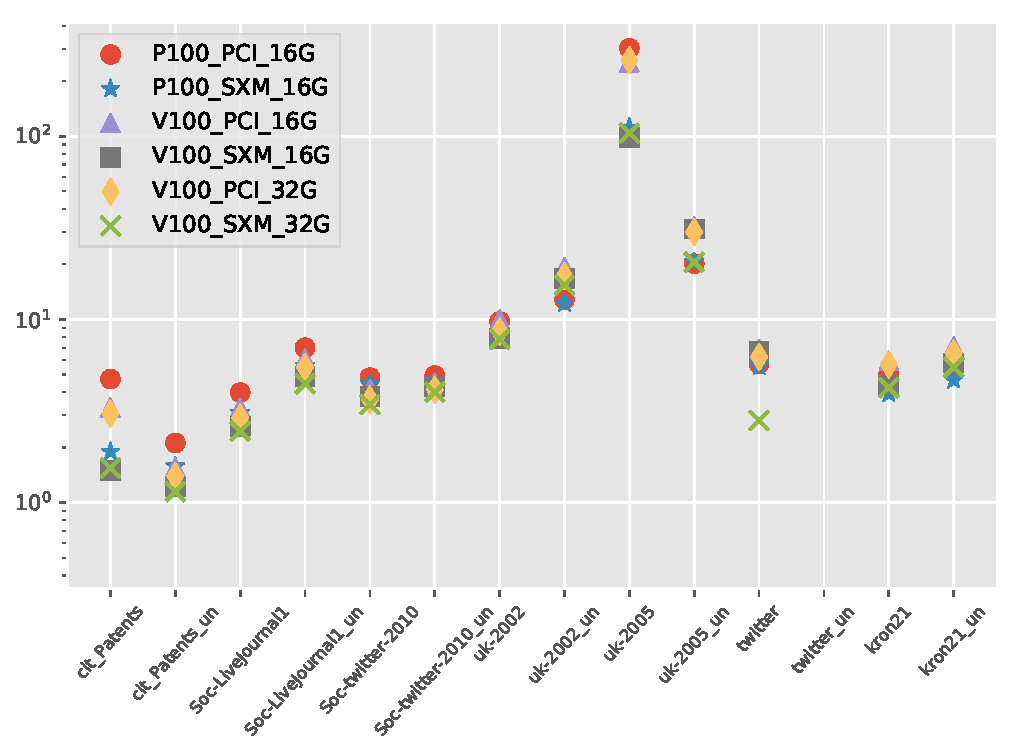
\includegraphics[width=.32\linewidth]{plots/log_GTEPS_G_BFS_Hornet.pdf}&
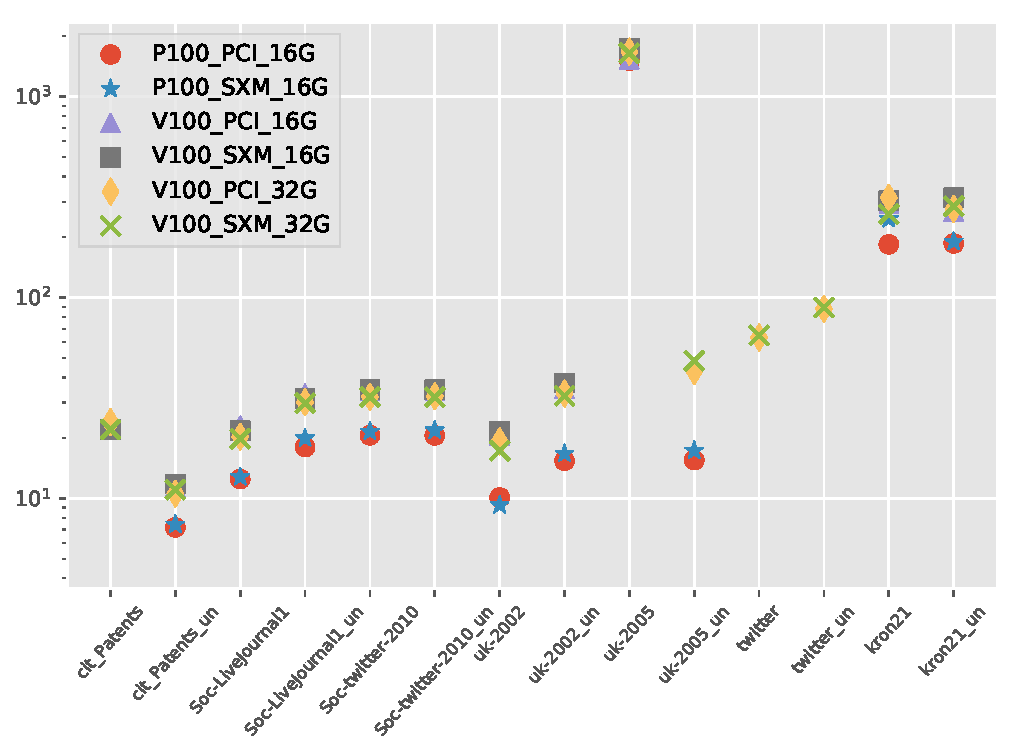
\includegraphics[width=.32\linewidth]{plots/log_GTEPS_G_BFS_Gunrock_Opt.pdf}&
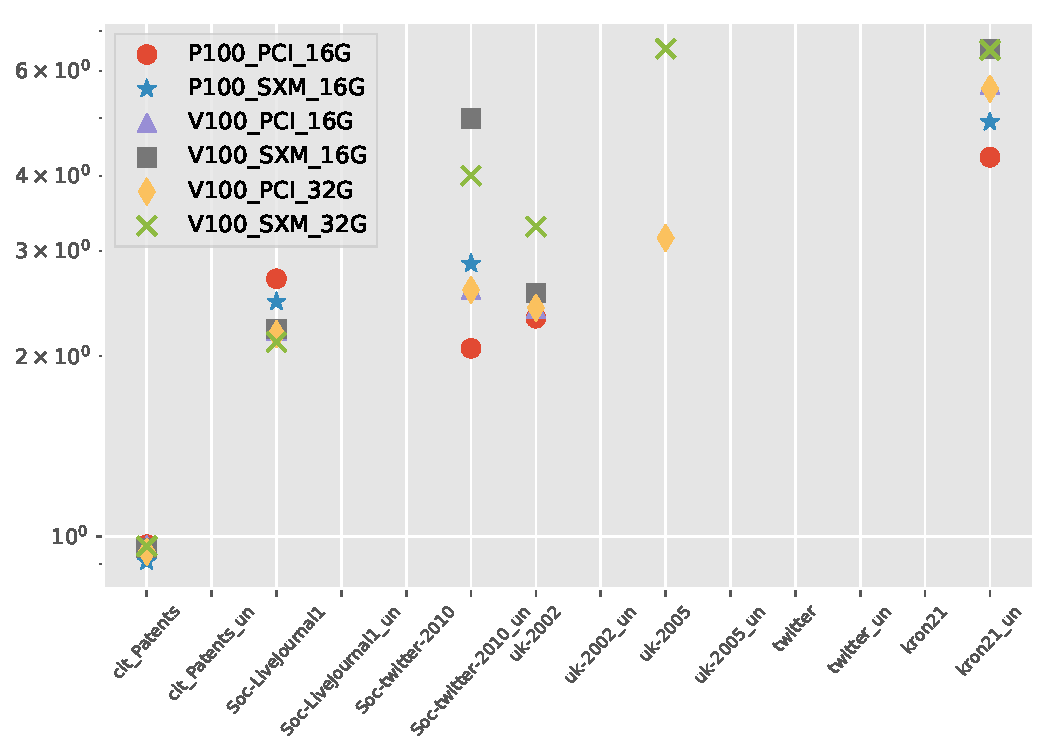
\includegraphics[width=.32\linewidth]{plots/log_GTEPS_G_BFS_cuGraph.pdf}\\[-1ex]
%&\mycaption{0.2} & \mycaption{0.2} & \mycaption{0.3}\\
\rowname{\small\textbf{PR}}
&
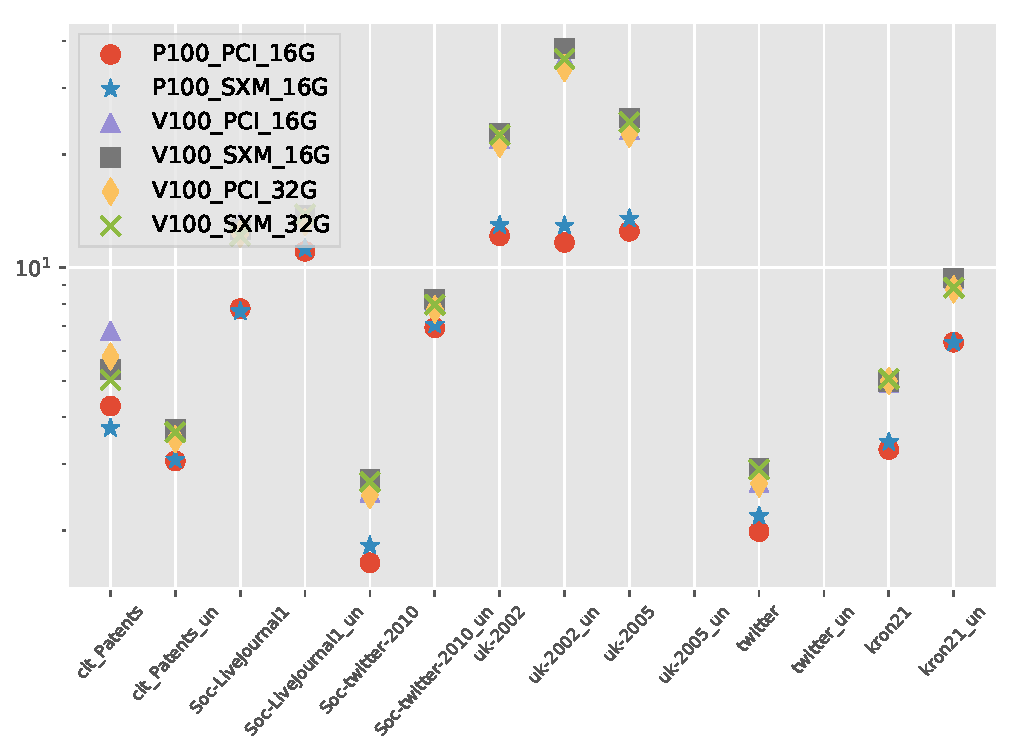
\includegraphics[width=.32\linewidth]{plots/log_GTEPS_G_PR_Hornet.pdf}&
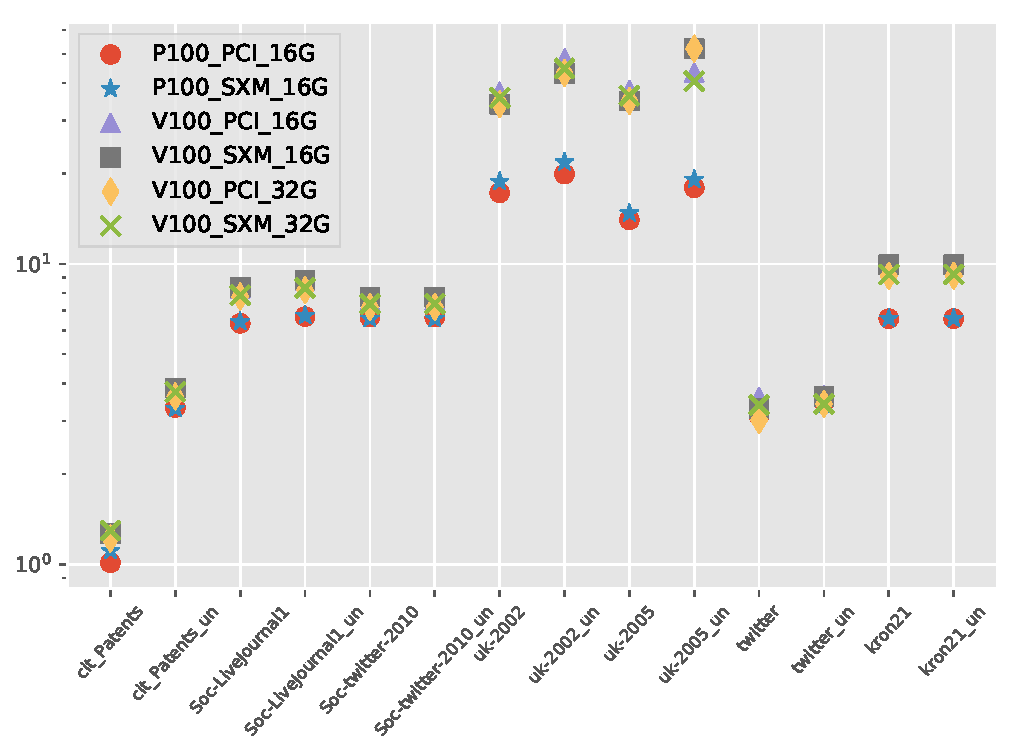
\includegraphics[width=.32\linewidth]{plots/log_GTEPS_G_PR_Gunrock_Opt.pdf}&
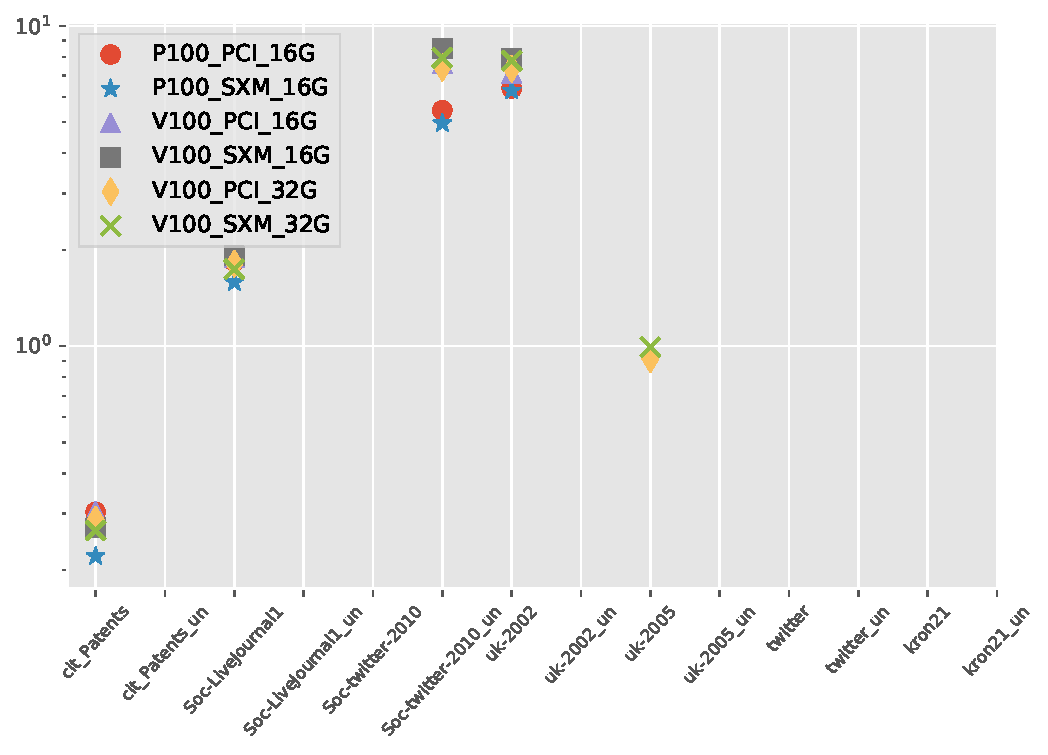
\includegraphics[width=.32\linewidth]{plots/log_GTEPS_G_PR_cuGraph.pdf}\\[-1ex]
%&\mycaption{0.5} & \mycaption{0.4} & \mycaption{0.6}%\\
\rowname{\small\textbf{BC}}&
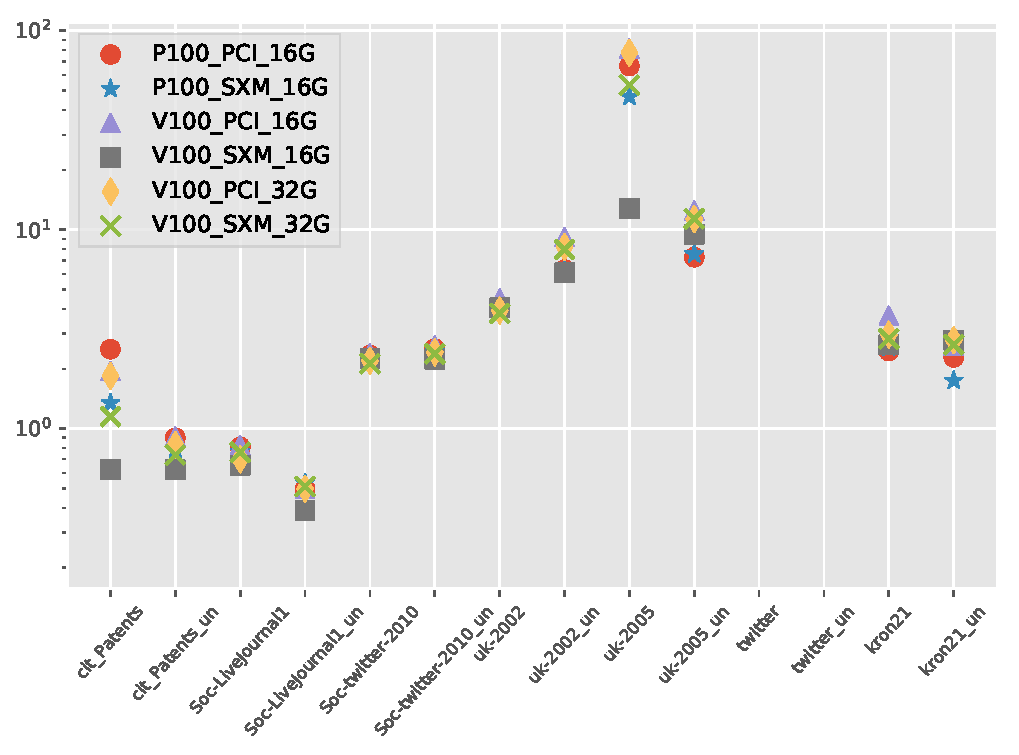
\includegraphics[width=.32\linewidth]{plots/log_GTEPS_G_BC_Hornet.pdf}&
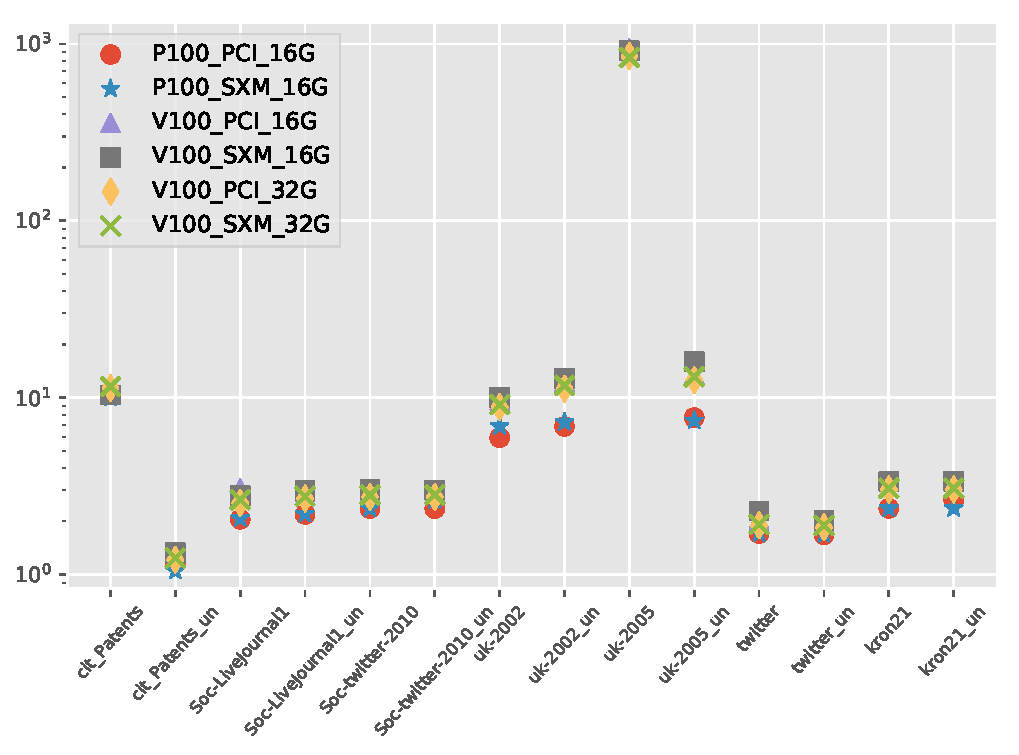
\includegraphics[width=.32\linewidth]{plots/log_GTEPS_G_BC_Gunrock_Opt.pdf}&
\includegraphics[width=.32\linewidth]{}\\[-1ex]
%&\mycaption{0.5} & \mycaption{0.4} & \mycaption{0.6}%\\
\rowname{\small\textbf{CC}}&
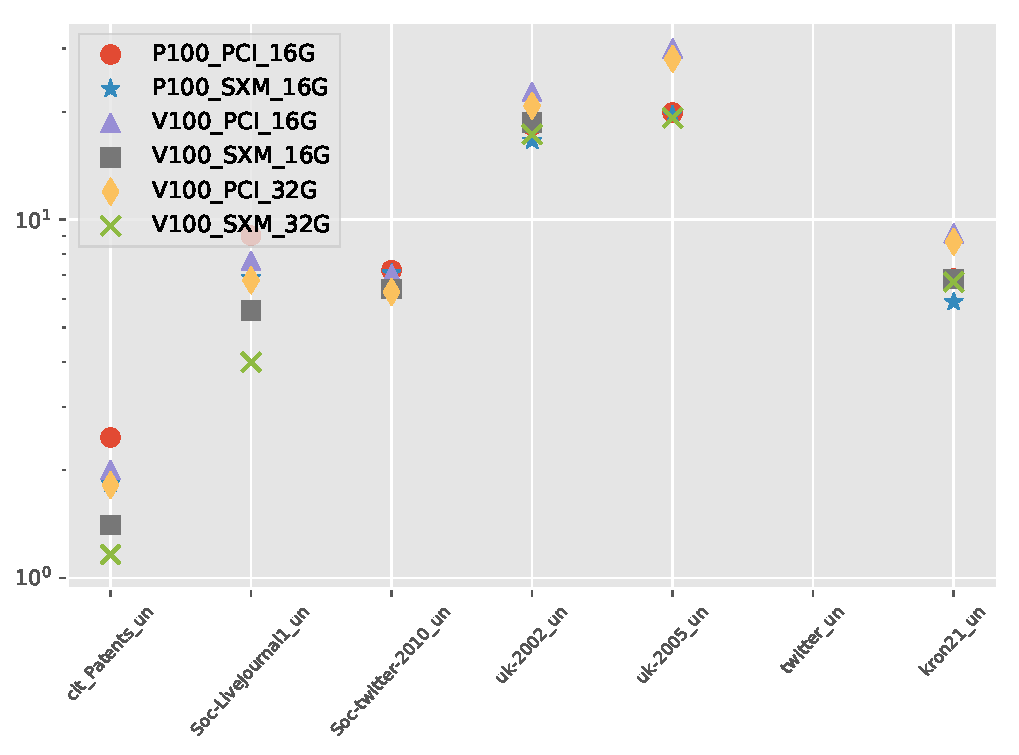
\includegraphics[width=.32\linewidth]{plots/log_GTEPS_G_CC_Hornet.pdf}&
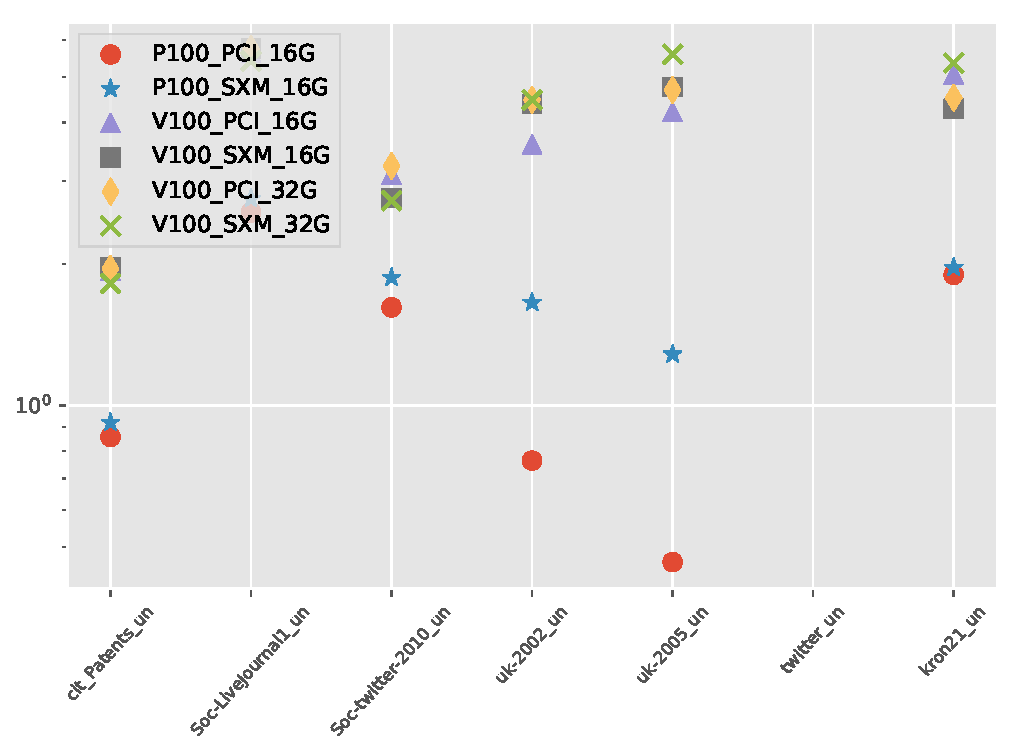
\includegraphics[width=.32\linewidth]{plots/log_GTEPS_G_CC_Gunrock_Def.pdf}&
\includegraphics[width=.23\linewidth]{}\\[-1ex]
%&\mycaption{0.5} & \mycaption{0.4} & \mycaption{0.6}%\\
\rowname{\small\textbf{TC}}&
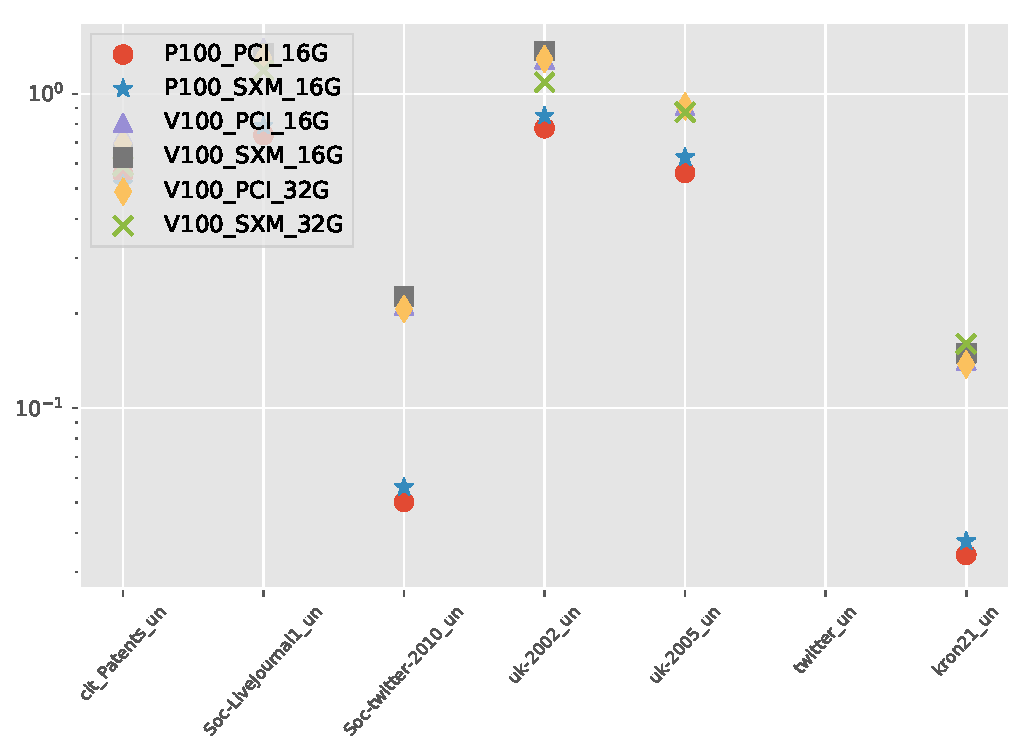
\includegraphics[width=.32\linewidth]{plots/log_GTEPS_G_TC_Hornet.pdf}&
\includegraphics[width=.32 \linewidth]{}&
\includegraphics[width=.32 \linewidth]{}\\[-1ex]
%&\mycaption{0.5} & \mycaption{0.4} & \mycaption{0.6}%\\
\end{tabular}
\caption{Logarithmic GTEPS of each benchmark with real world and synthetic graph(s) in Hornet, Gunrock, and cuGraph}%
\label{figure1}
\end{figure}

\begin{figure}
\settoheight{\tempdima}{\includegraphics[width=.3\linewidth]{example-image-a}}%
\centering\begin{tabular}{@{}c@{ }c@{ }c@{ }}
&\textbf{PCI} & \textbf{SXM} &
\rowname{(P100-16GB) \small\textbf{BFS}}&
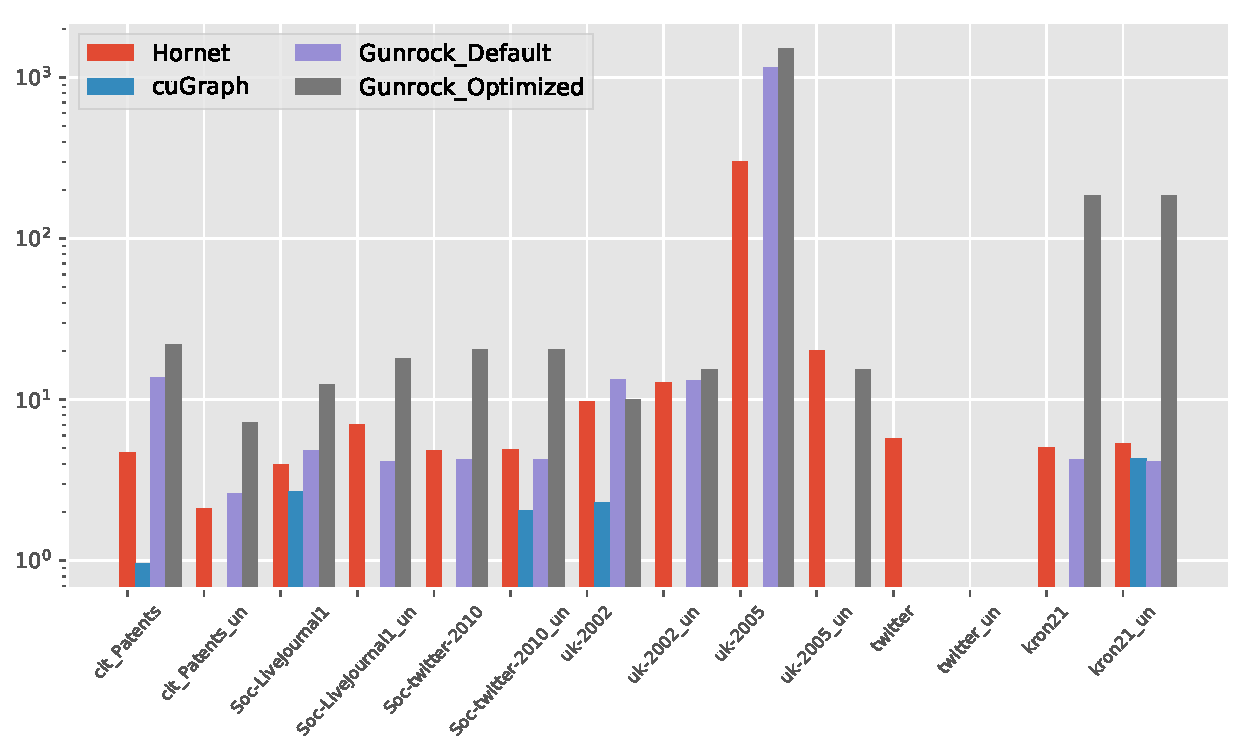
\includegraphics[width=.45\linewidth]{plots/log_GTEPS_G_BFS_PP16.pdf}&
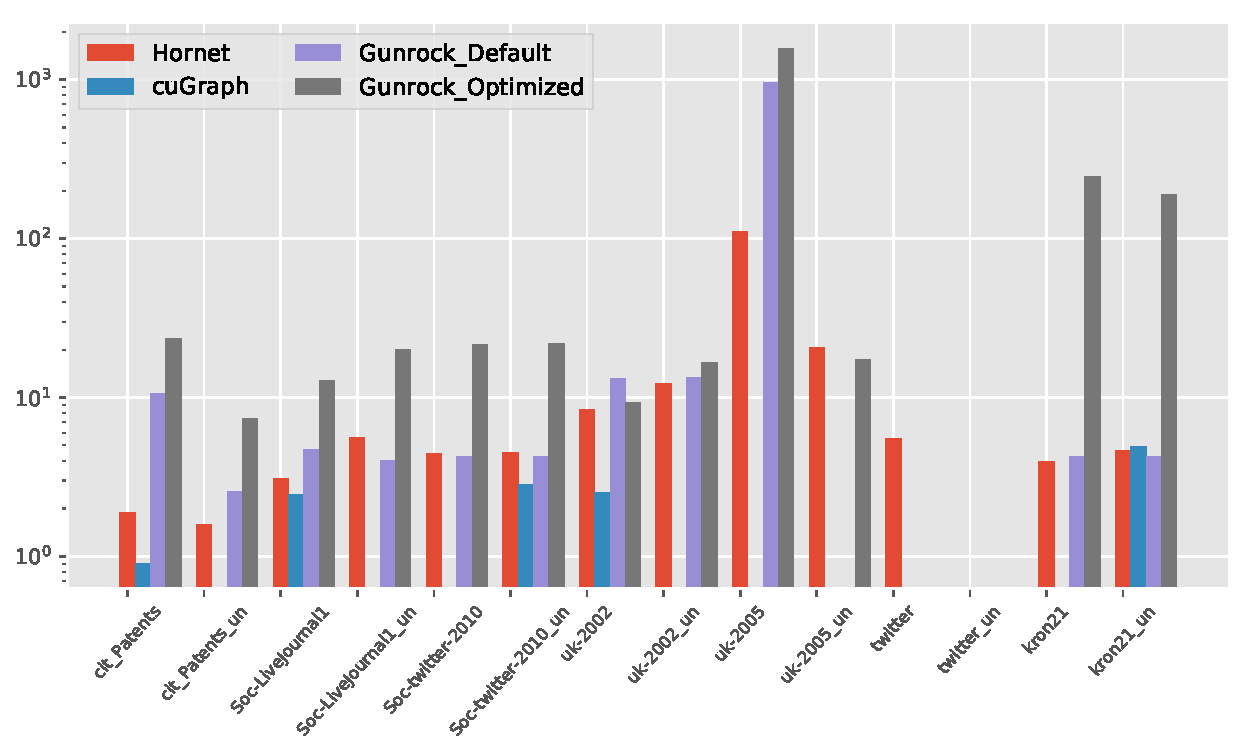
\includegraphics[width=.45\linewidth]{plots/log_GTEPS_G_BFS_PS16.pdf}\\[-1ex]
\rowname{(V100-16GB) \small\textbf{BFS}}&
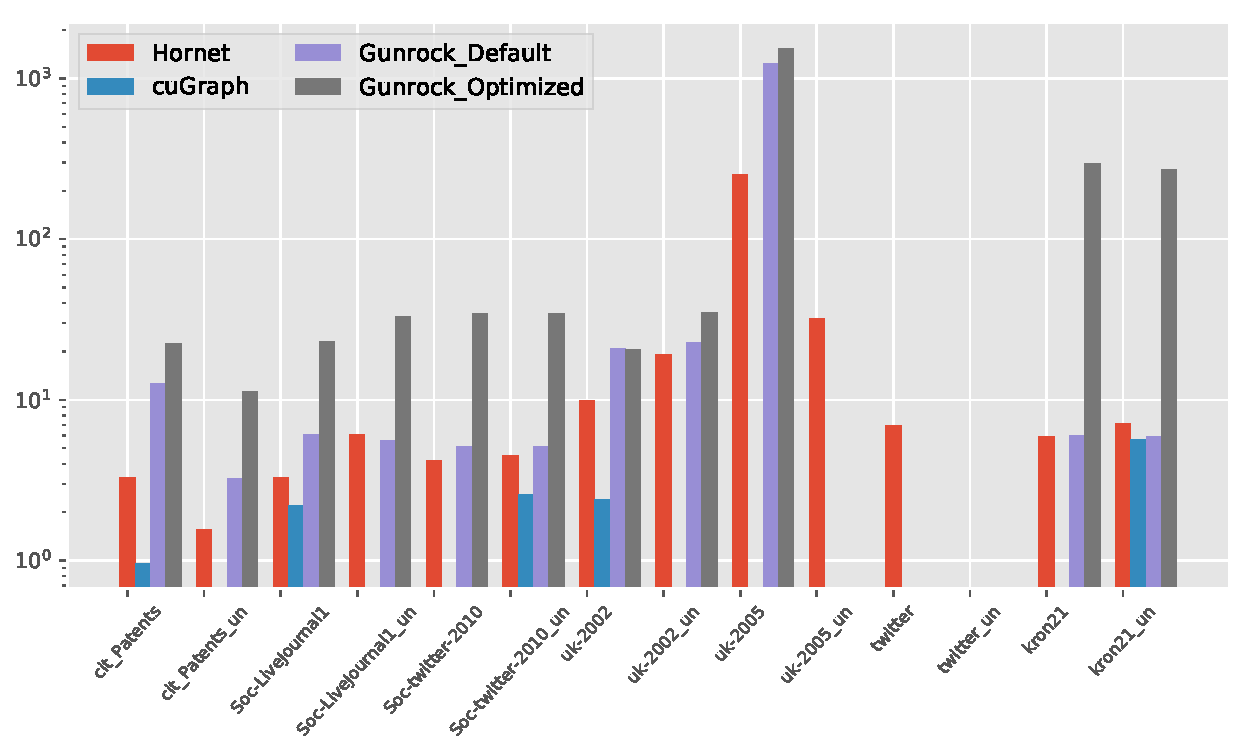
\includegraphics[width=.45\linewidth]{plots/log_GTEPS_G_BFS_VP16.pdf}&
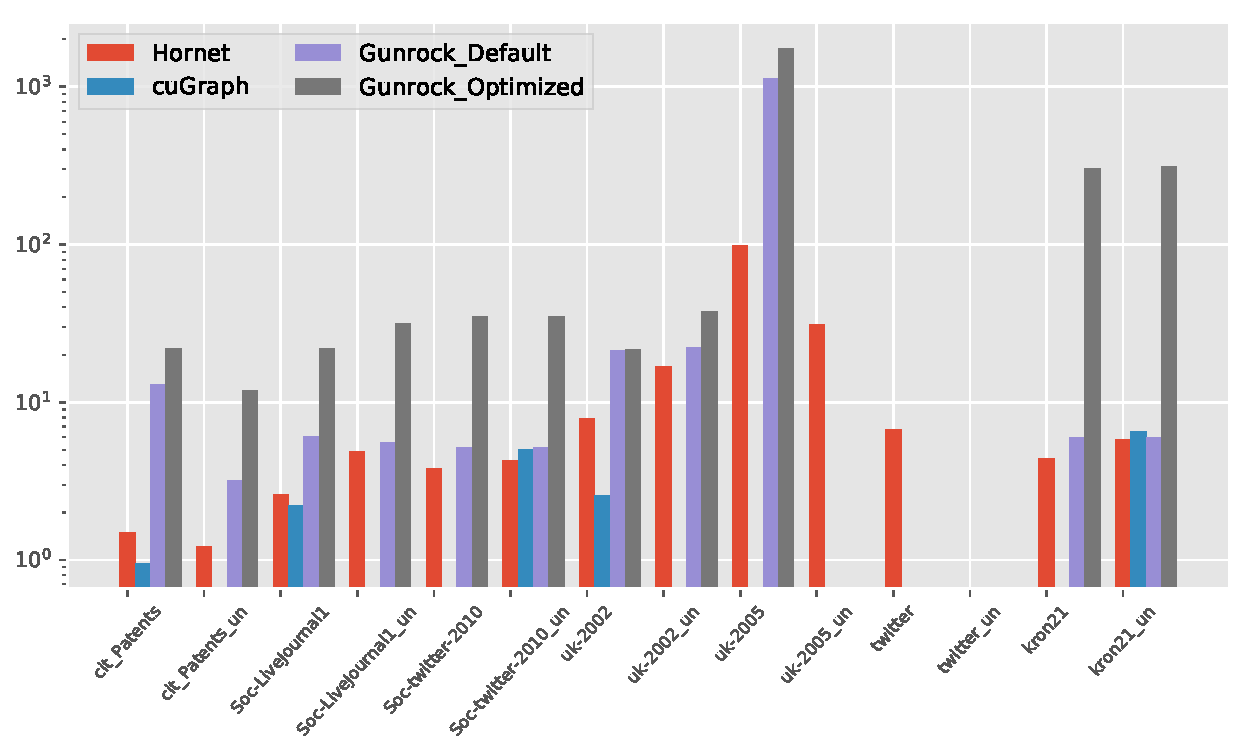
\includegraphics[width=.45\linewidth]{plots/log_GTEPS_G_BFS_VS16.pdf}\\[-1ex]
\rowname{(V100-32GB) \small\textbf{BFS}}&
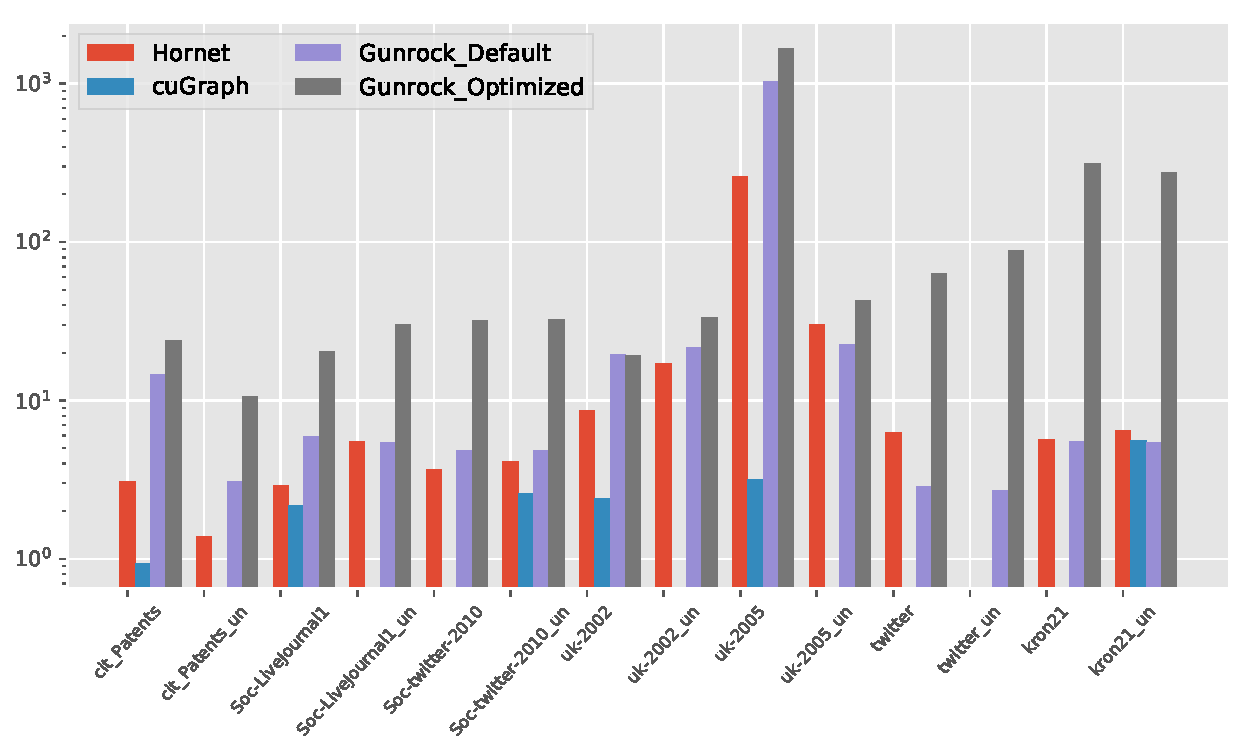
\includegraphics[width=.45\linewidth]{plots/log_GTEPS_G_BFS_VP32.pdf}&
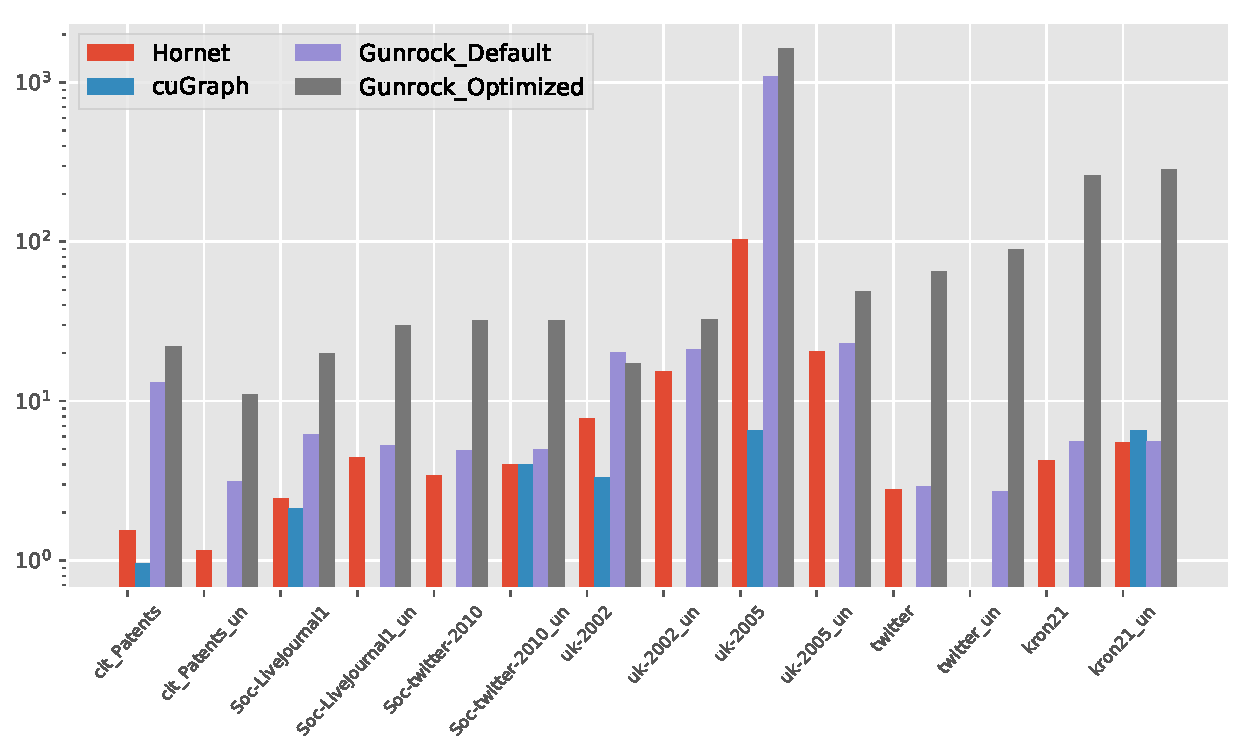
\includegraphics[width=.45\linewidth]{plots/log_GTEPS_G_BFS_VS32.pdf}\\[-1ex]
\rowname{(P100-16GB) \small\textbf{PR}}&
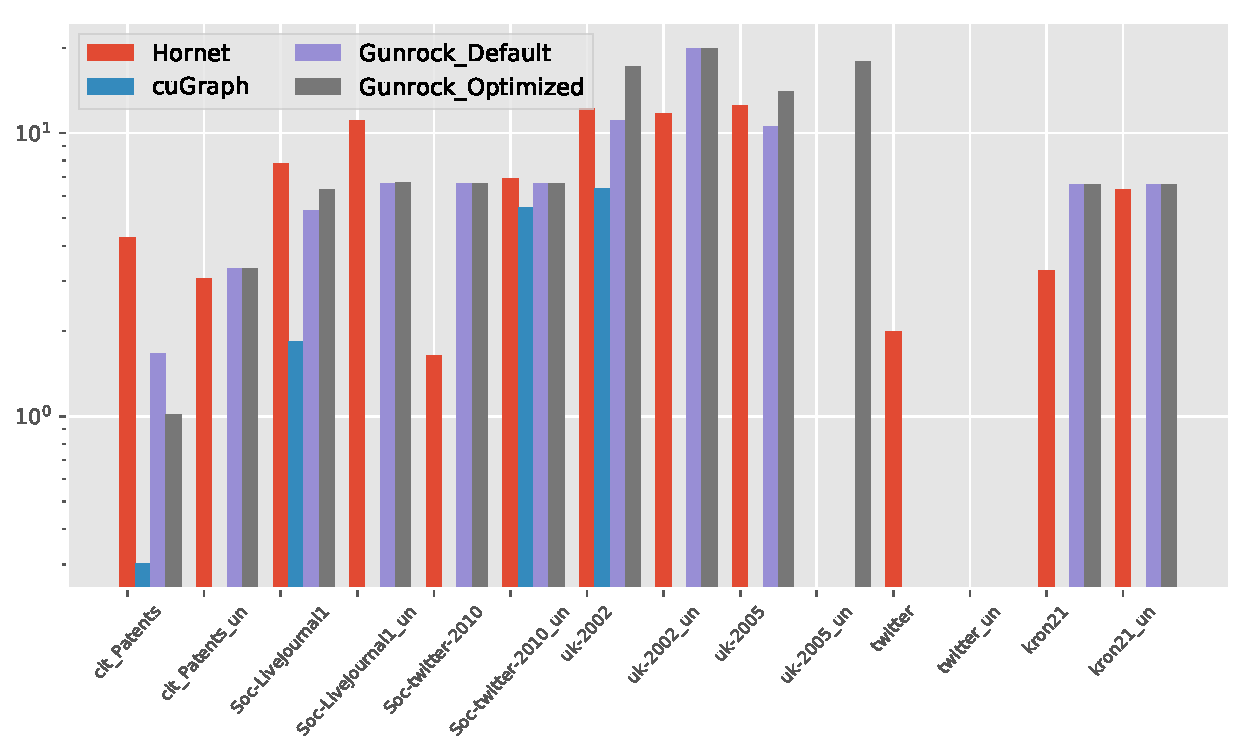
\includegraphics[width=.45\linewidth]{plots/log_GTEPS_G_PR_PP16.pdf}&
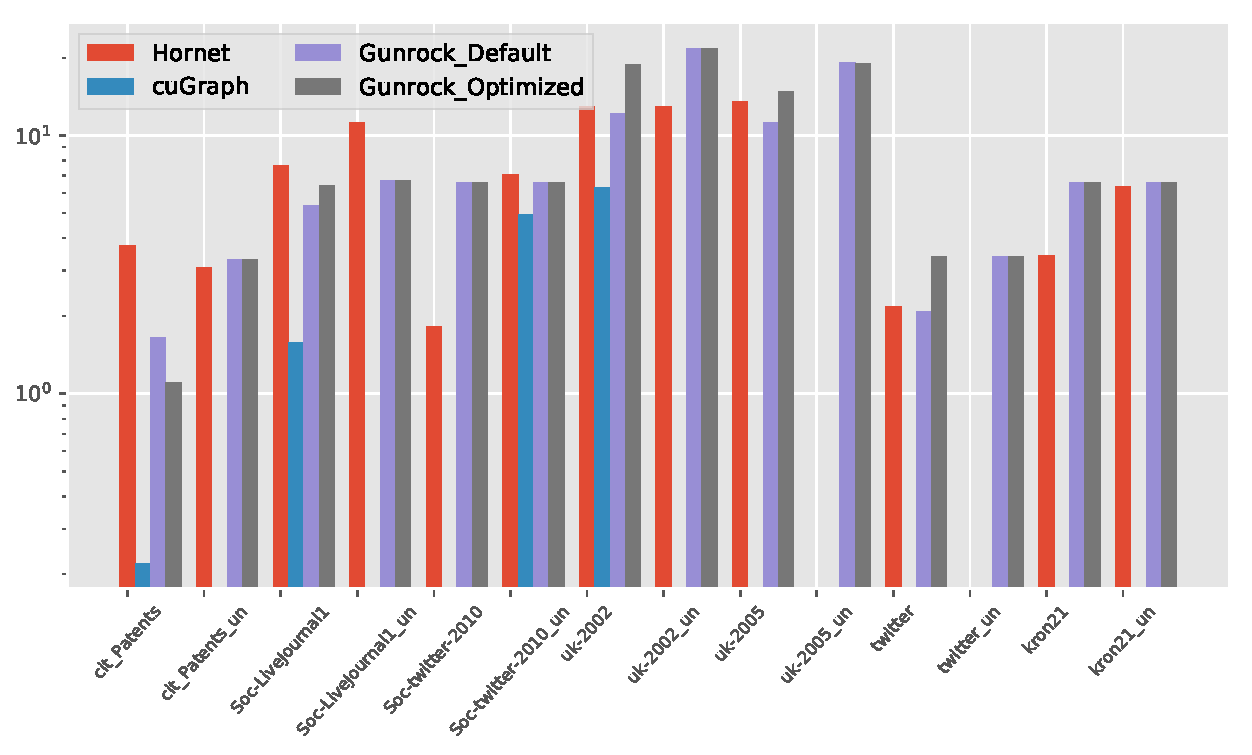
\includegraphics[width=.45\linewidth]{plots/log_GTEPS_G_PR_PS16.pdf}\\[-1ex]
\rowname{(V100-16GB) \small\textbf{PR}}&
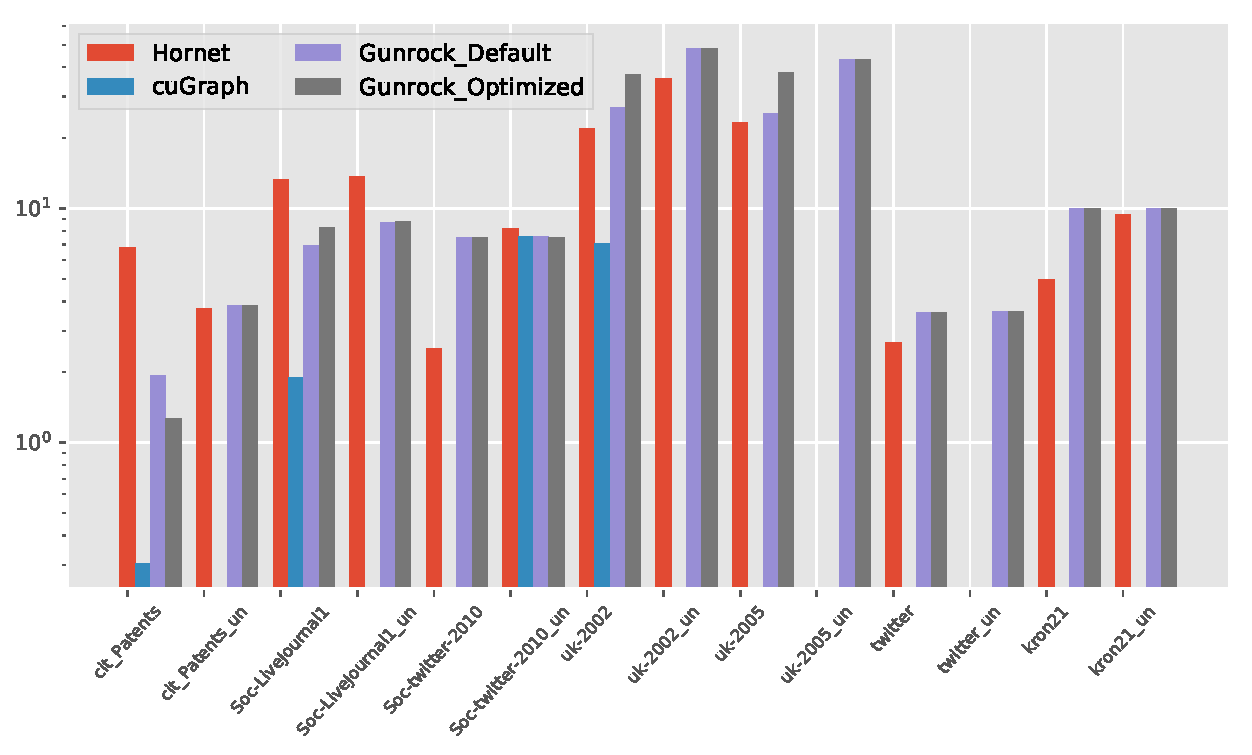
\includegraphics[width=.45\linewidth]{plots/log_GTEPS_G_PR_VP16.pdf}&
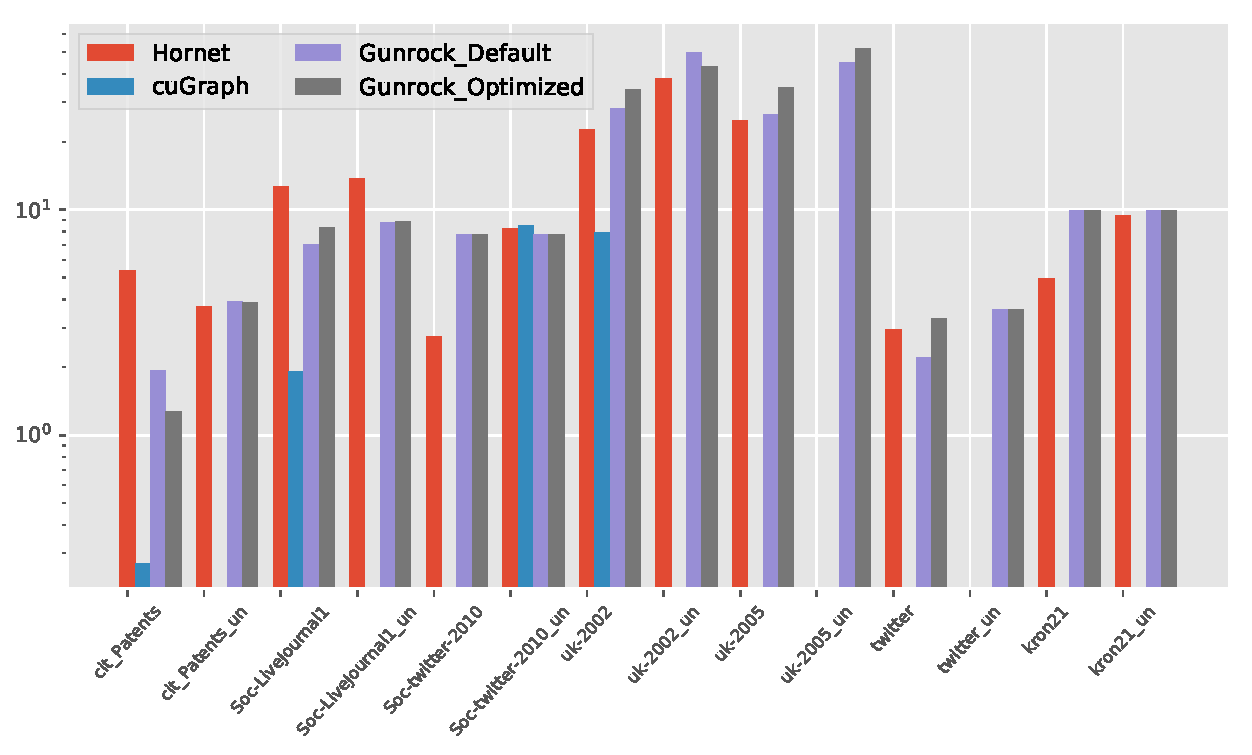
\includegraphics[width=.45\linewidth]{plots/log_GTEPS_G_PR_VS16.pdf}\\[-1ex]
\rowname{(V100-32GB) \small\textbf{PR}}&
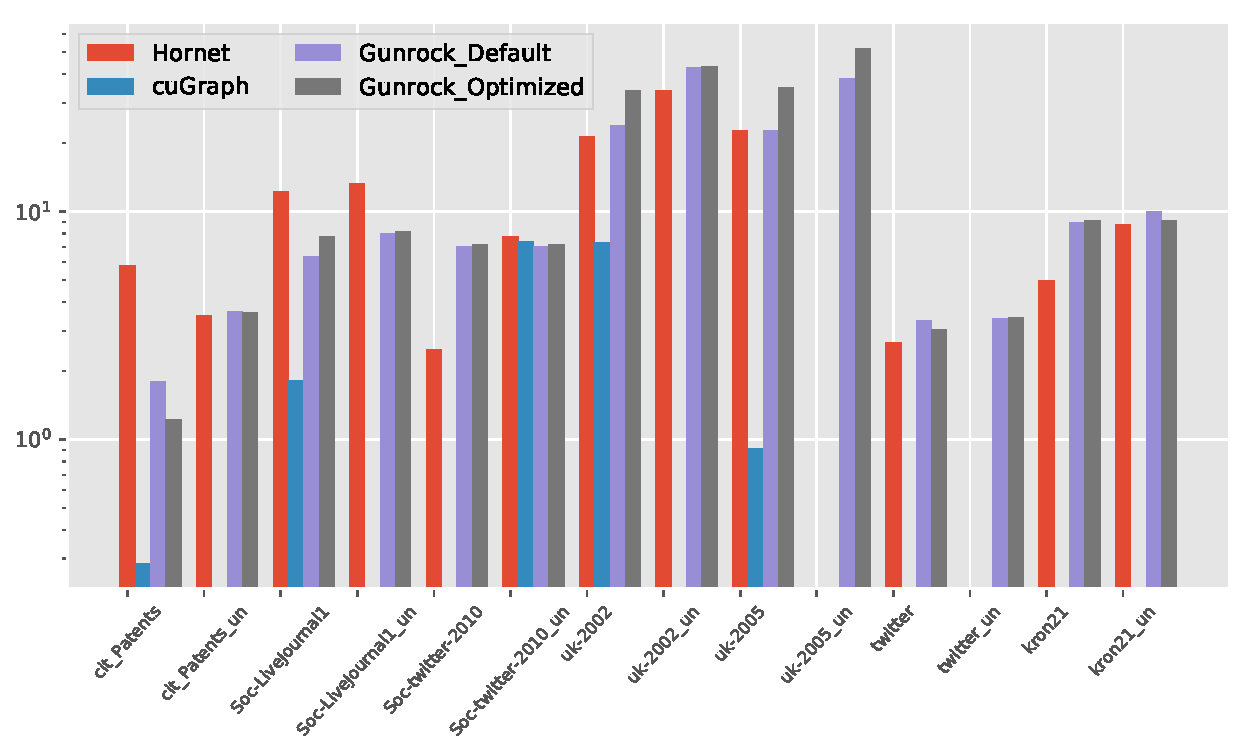
\includegraphics[width=.45\linewidth]{plots/log_GTEPS_G_PR_VP32.pdf}&
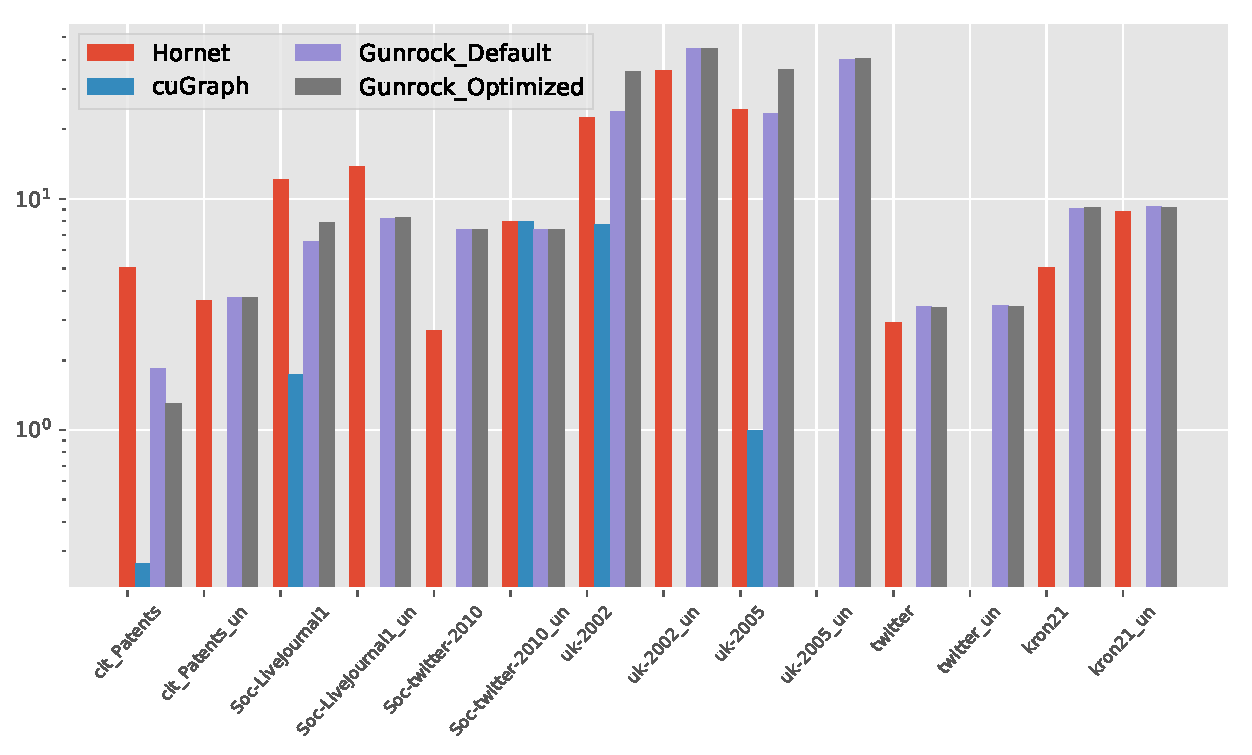
\includegraphics[width=.45\linewidth]{plots/log_GTEPS_G_PR_VS32.pdf}\\[-1ex]
\rowname{(P100-16GB) \small\textbf{BC}}&
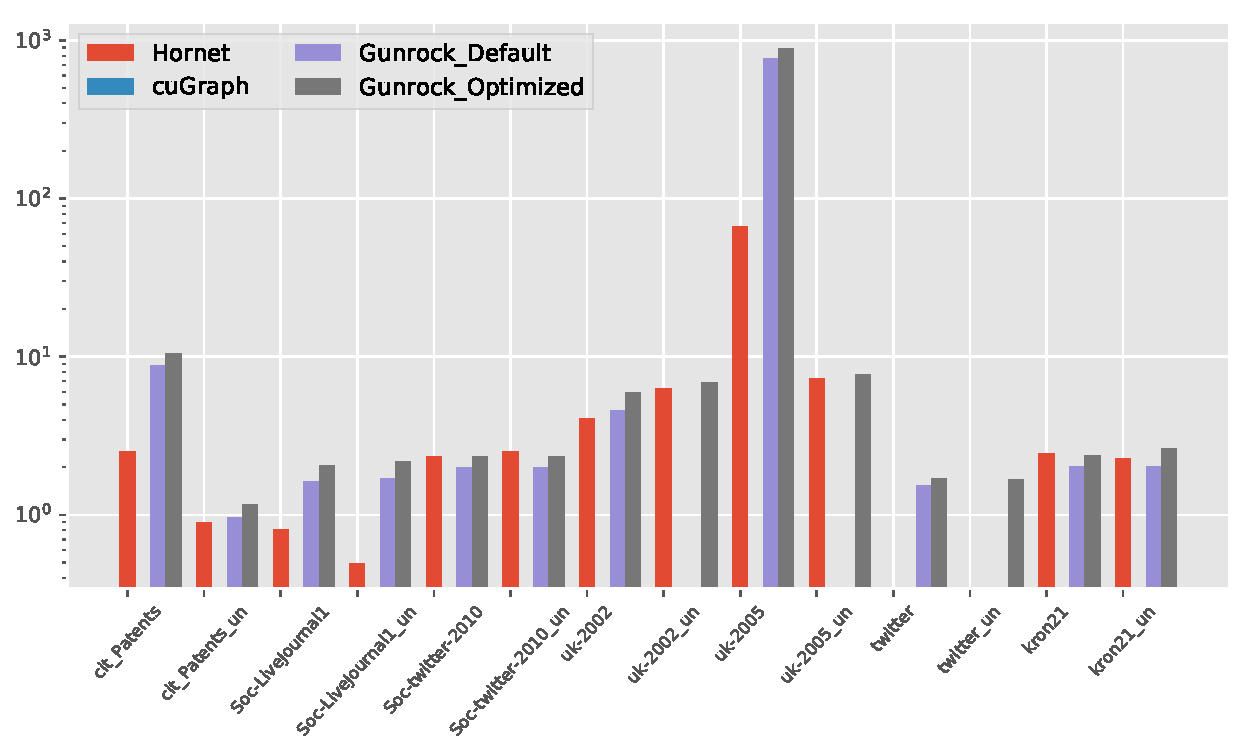
\includegraphics[width=.45\linewidth]{plots/log_GTEPS_G_BC_PP16.pdf}&
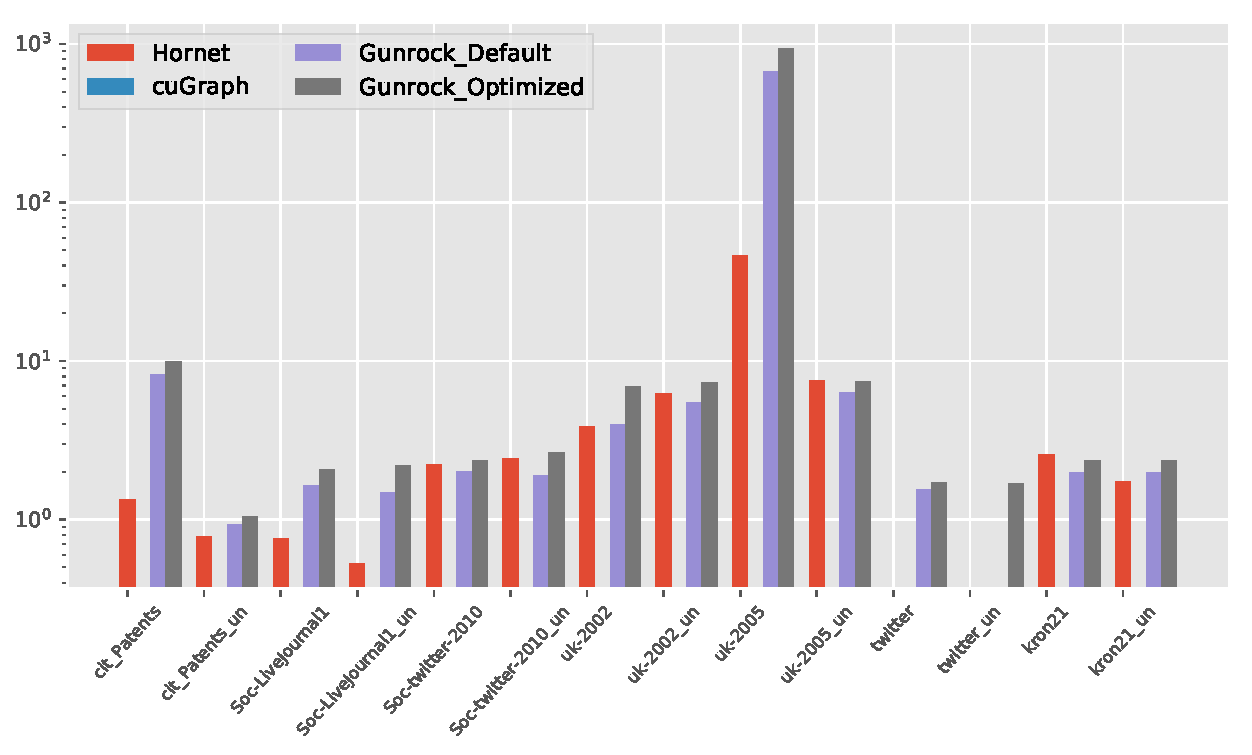
\includegraphics[width=.45\linewidth]{plots/log_GTEPS_G_BC_PS16.pdf}\\[-1ex]
\rowname{(V100-16GB) \small\textbf{BC}}&
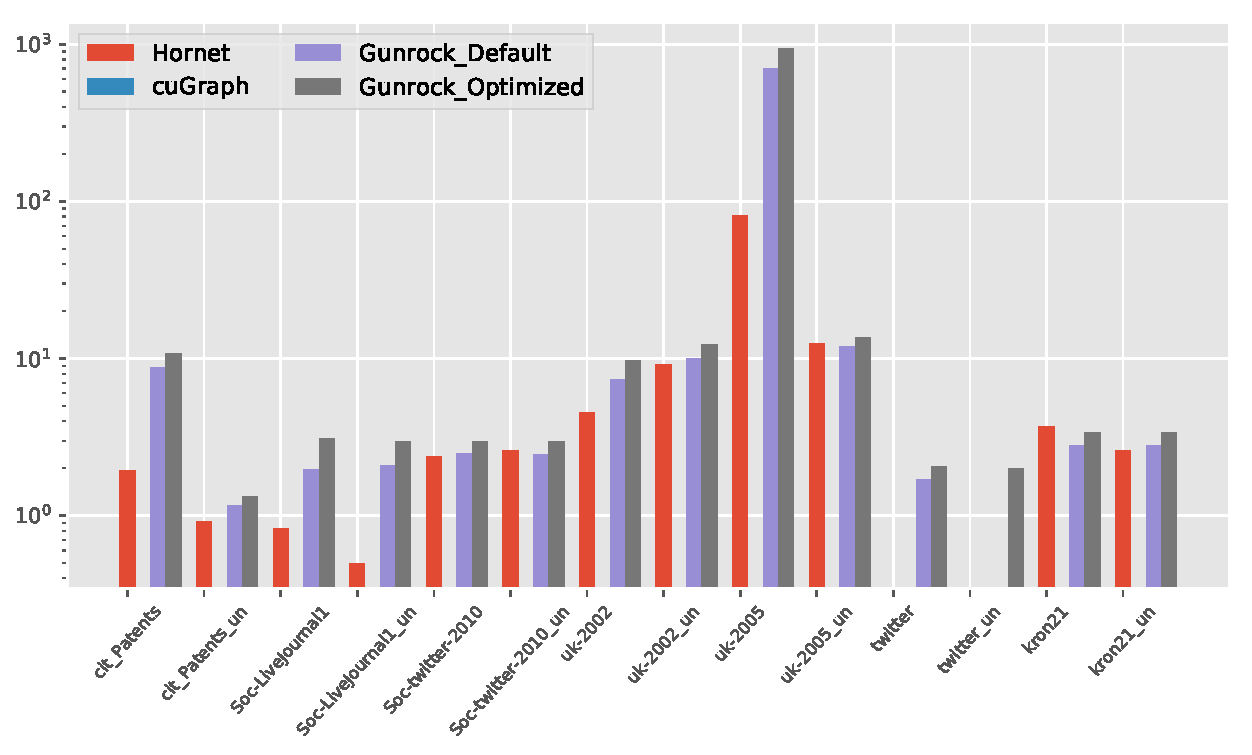
\includegraphics[width=.45\linewidth]{plots/log_GTEPS_G_BC_VP16.pdf}&
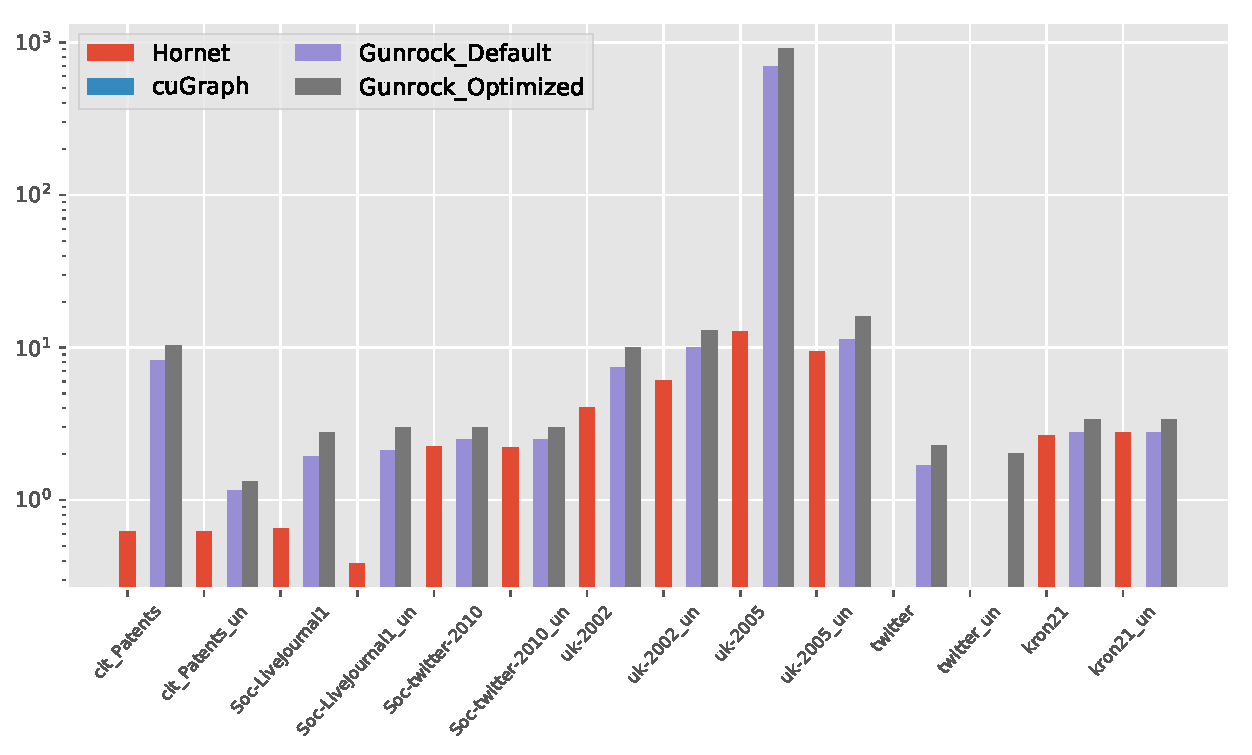
\includegraphics[width=.45\linewidth]{plots/log_GTEPS_G_BC_VS16.pdf}\\[-1ex]
\rowname{(V100-32GB) \small\textbf{BC}}&
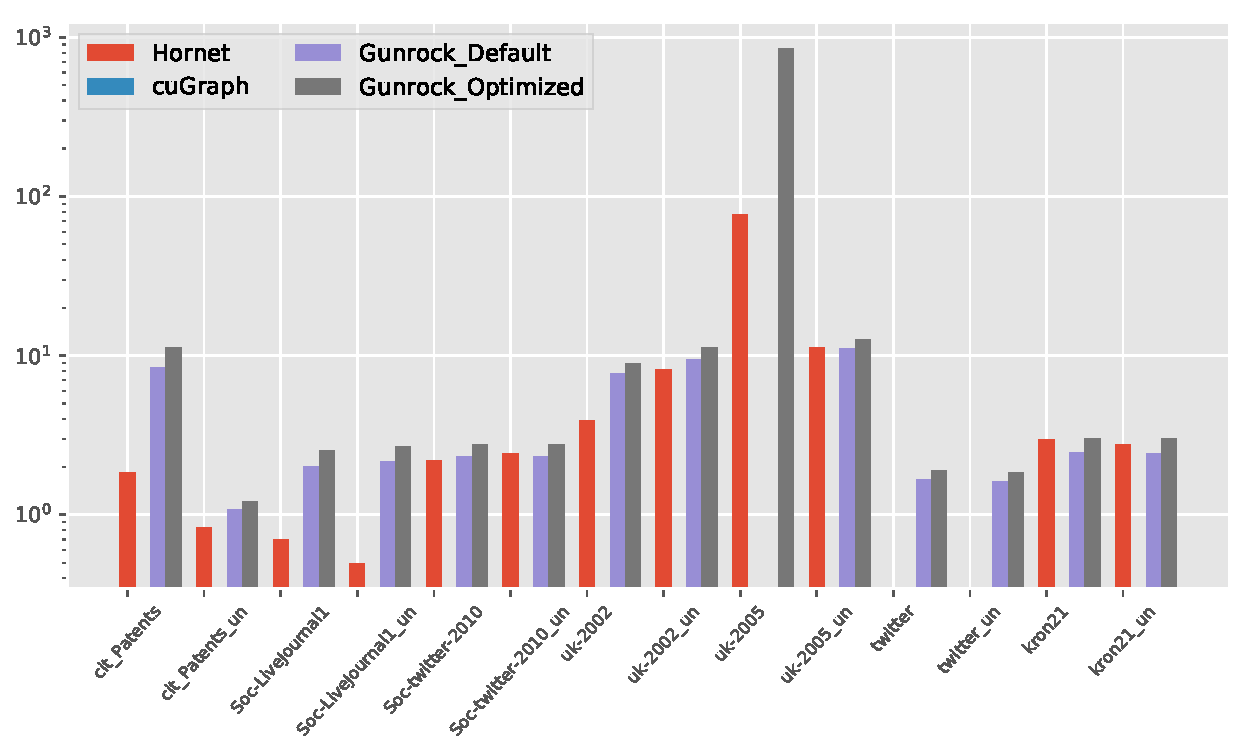
\includegraphics[width=.45\linewidth]{plots/log_GTEPS_G_BC_VP32.pdf}&
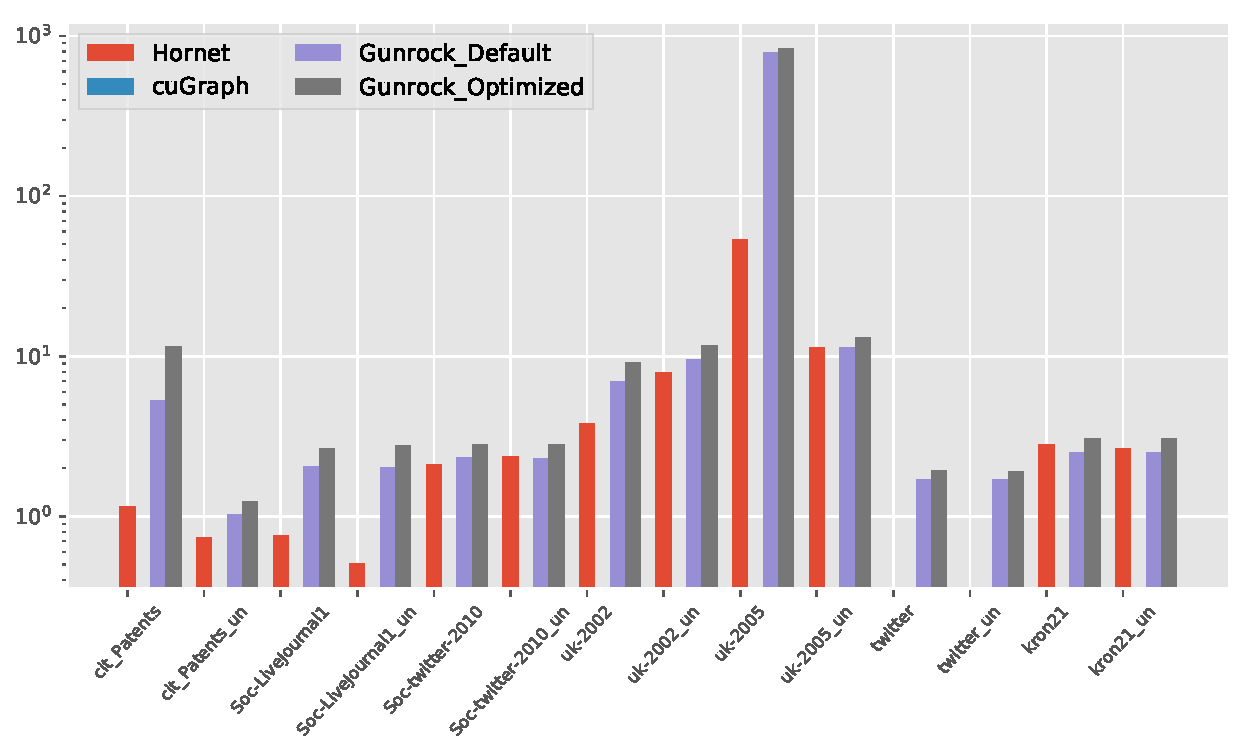
\includegraphics[width=.45\linewidth]{plots/log_GTEPS_G_BC_VS32.pdf}\\[-1ex]
\end{tabular}
\caption{GTEPS of benchmarks BFS, PR, BC, CC, and TC in six different GPU systems. Traveral algorithms such as BFS are executed with the largest degree node as a root. Some benchmarks are available in all frameworks, such as CC in cuGraph. A few computations are not completed and not shown to OOM(Out-of-memory)}%
\label{fig:GTEPS_ALL}
\end{figure}

\begin{figure}
\settoheight{\tempdima}{\includegraphics[width=.3\linewidth]{example-image-a}}%
\centering\begin{tabular}{@{}c@{ }c@{ }c@{ }} 
& \textbf{PCI} & \textbf{SXM} &
\rowname{(P100-16GB) \small\textbf{CC}}&
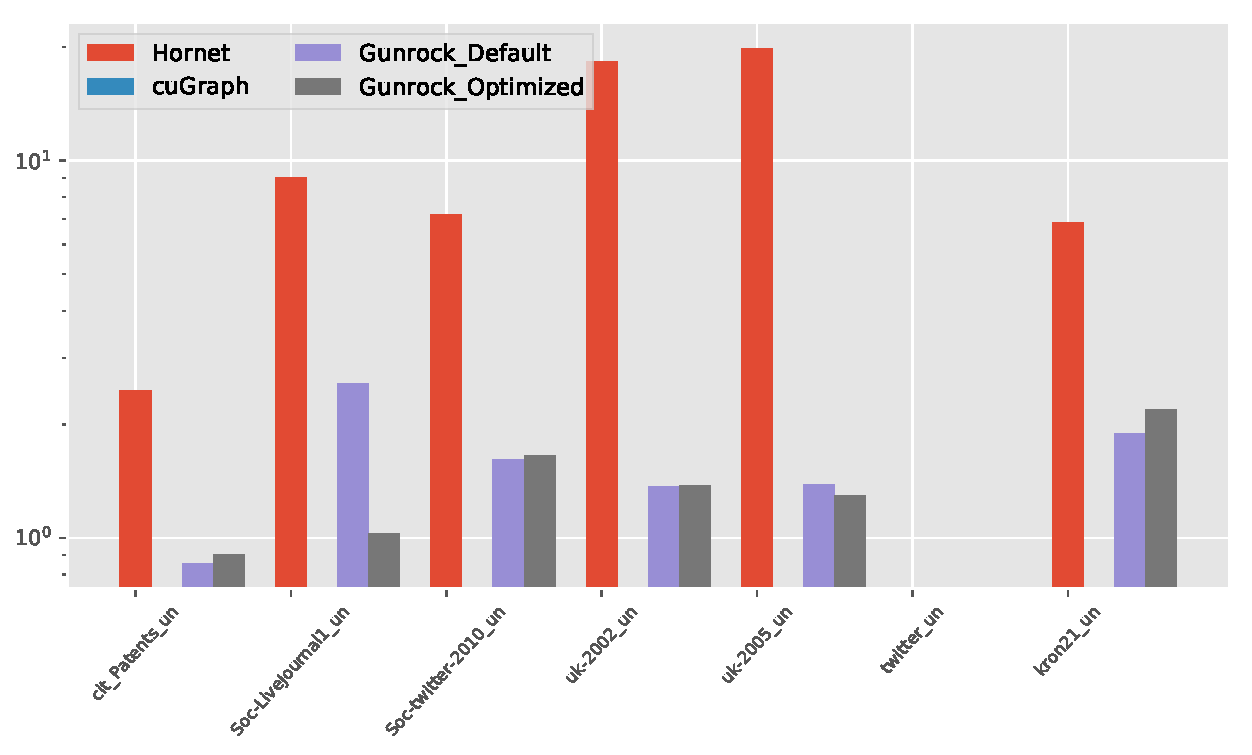
\includegraphics[width=.4\linewidth]{plots/log_GTEPS_G_CC_PP16.pdf}&
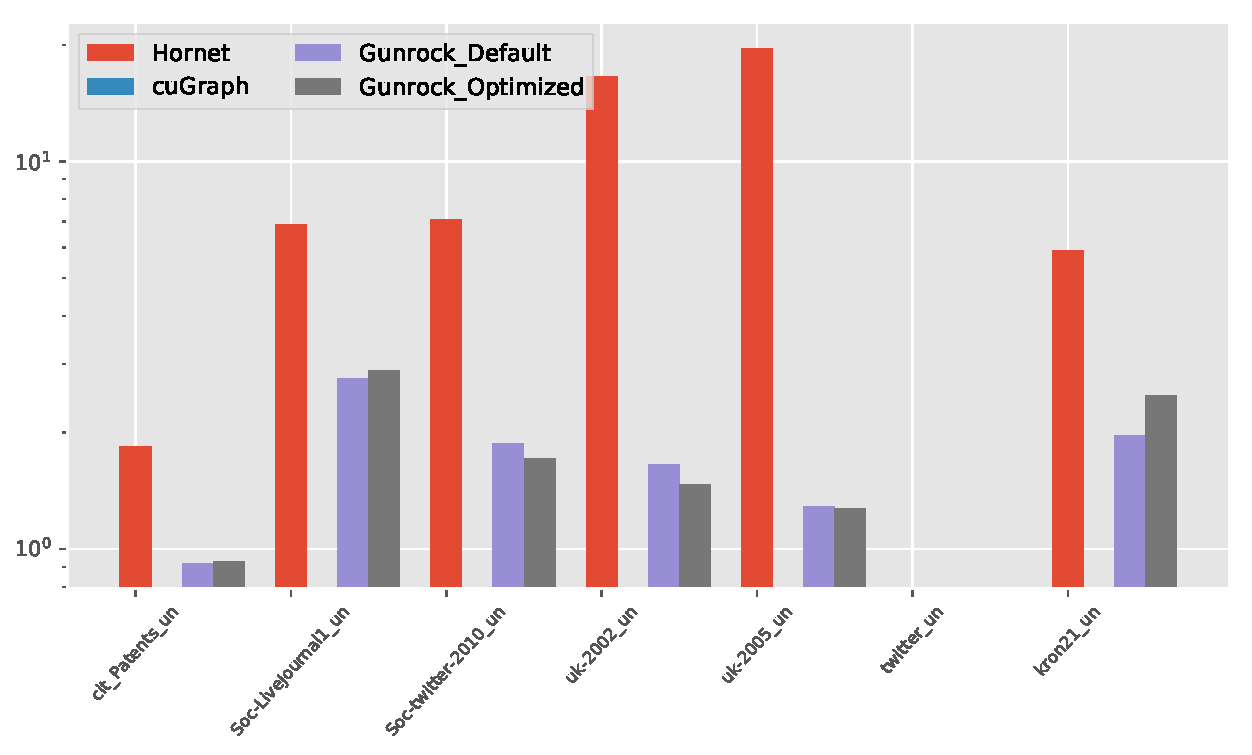
\includegraphics[width=.4\linewidth]{plots/log_GTEPS_G_CC_PS16.pdf}\\[-1ex]
\rowname{(V100-16GB) \small\textbf{CC}}&
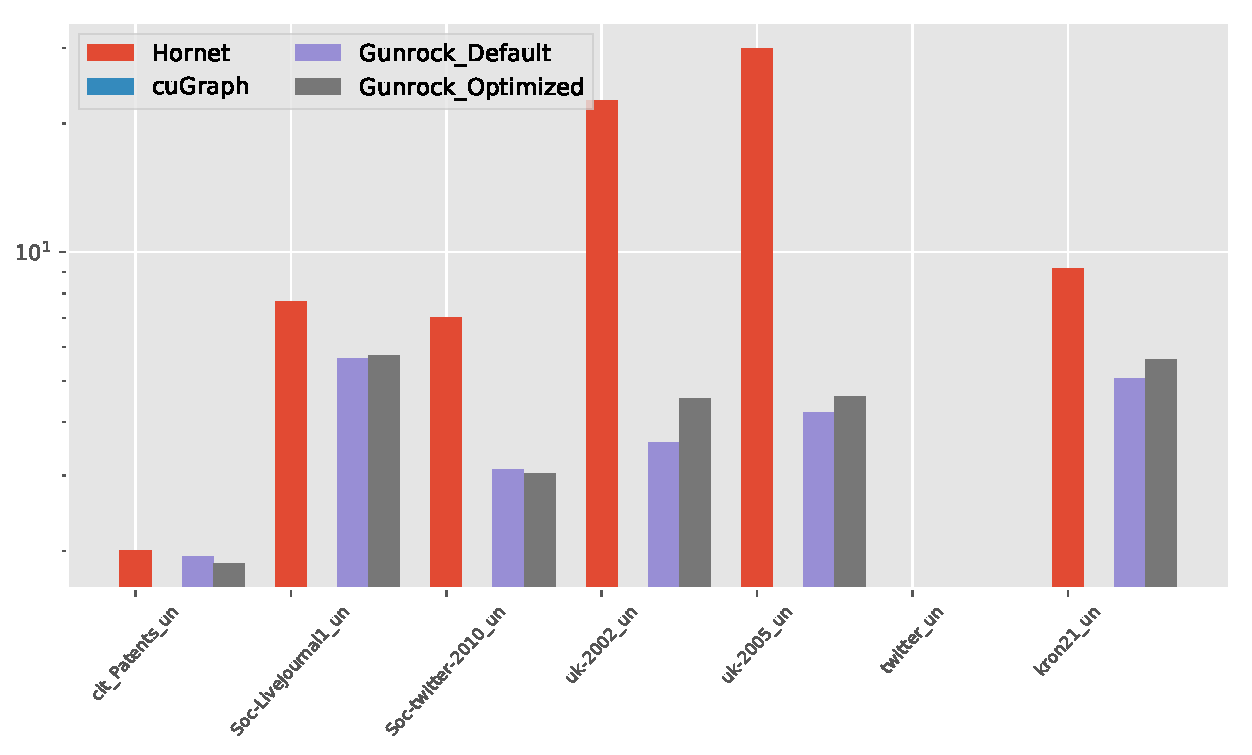
\includegraphics[width=.4\linewidth]{plots/log_GTEPS_G_CC_VP16.pdf}&
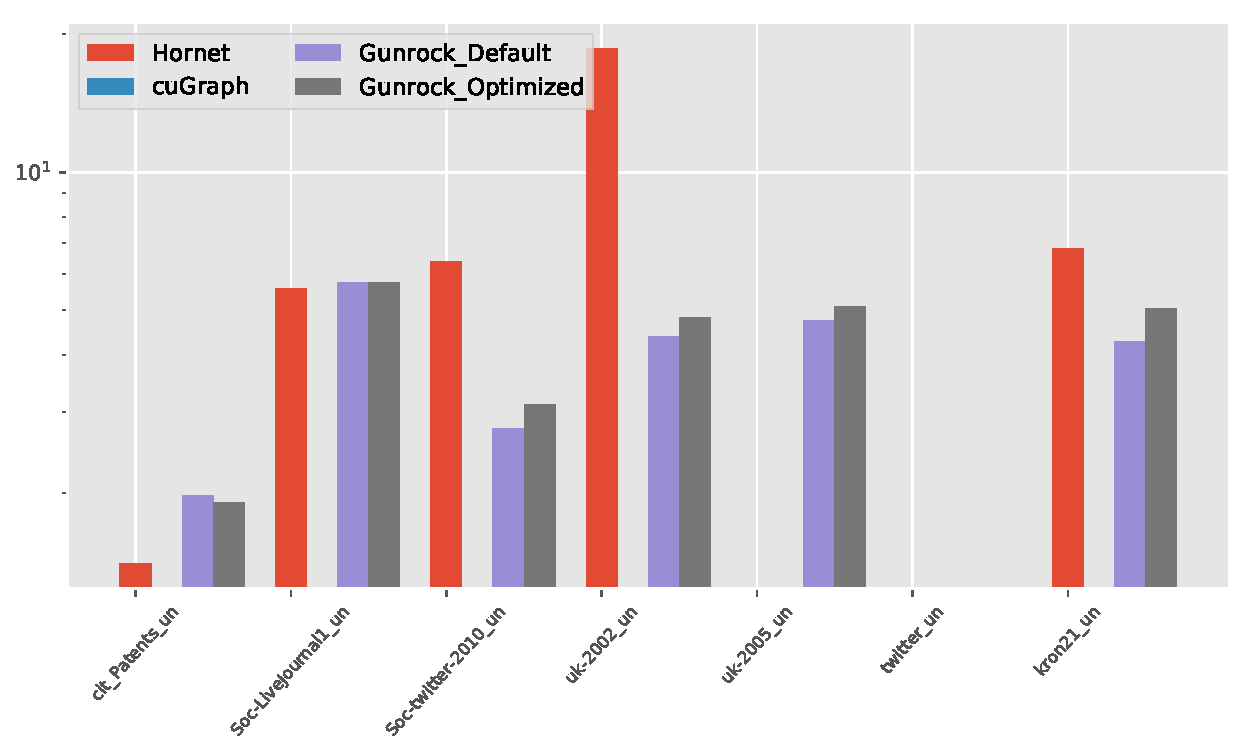
\includegraphics[width=.4\linewidth]{plots/log_GTEPS_G_CC_VS16.pdf}\\[-1ex]
\rowname{(V100-32GB) \small\textbf{CC}}&
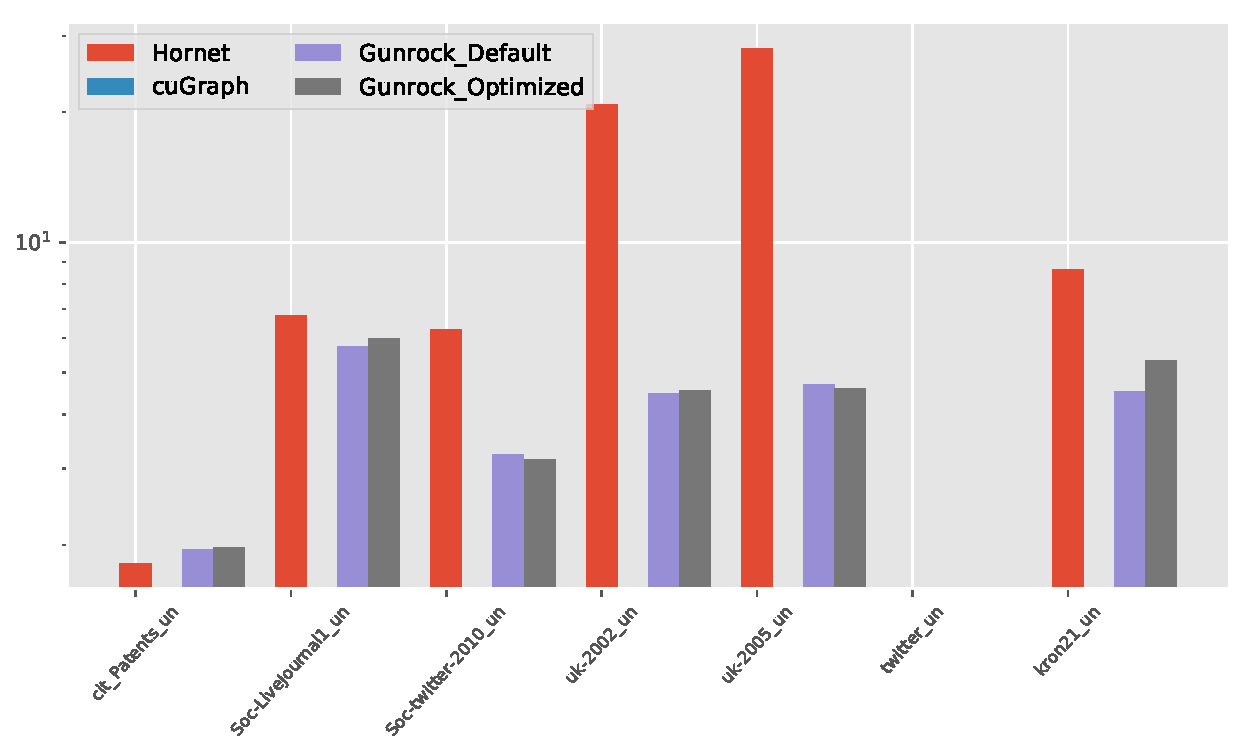
\includegraphics[width=.4\linewidth]{plots/log_GTEPS_G_CC_VP32.pdf}&
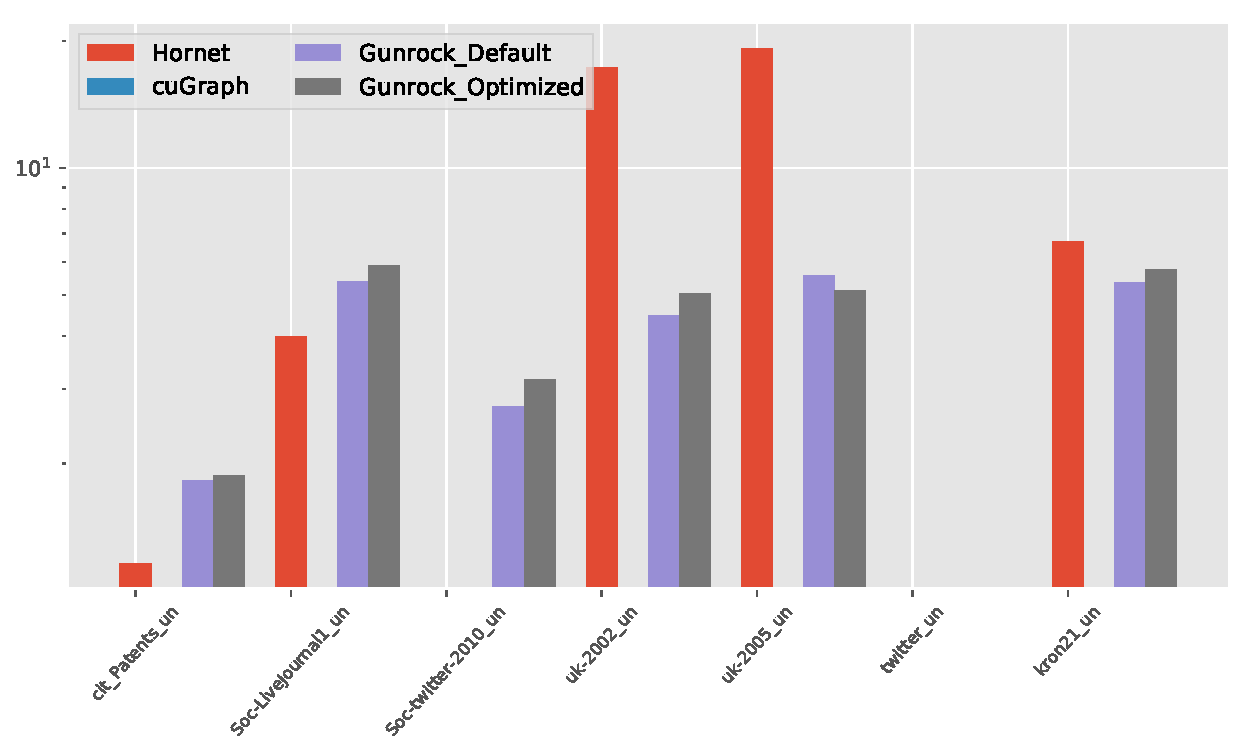
\includegraphics[width=.4\linewidth]{plots/log_GTEPS_G_CC_VS32.pdf}\\[-1ex]
\end{tabular}
\caption{[TBD] TC cuGraph results will be added}%
\label{fig:GTEPS_CC}
\end{figure}

We configured the frameworks with appropriate parameters for the functionality we evaluated. For instance, for Gunrock, we obtained results using both tuned and default parallelization options. 

For each case the operating systems, device driver types, and the versions of each are identical. As mentioned in \ref{sec:experiment-setup}, performance effects as a result of CPU differences are minimal since the measurement of computation time is only conducted on the GPU side. However, any processor-specific optimizations in the driver might affect performance. Note that the CPU types are different with respect to form factor and cache size; all of these differences are encapsulated in the general interconnect types, \emph{i.e.}, PCI-E and SXM, in the rest of this section.

 \subsection{Breadth First Search}
%[Euna] cuGraph BFS uses BLAS? not traversal?
%[Euna] Gunrock BFS is faster because of direction optimized implementation? refer to "four optimization strategies for graph traversal"
For most cases we found that cuGraph, the only BLAS based implementation, was slower than the vertex-centric implementation. In some cases it was up to $4 \times$ slower than Hornet and $20\times$ slower than Gunrock's faster implementation with parallelization options. Gunrock's BFS utilizes the popular bottom-up BFS scheme which is an algorithmic optimization available for vertex-centric algorithms that is not available for BLAS based implementations.
 
% Hornet's vertex-centric BFS algorithm has comparable performance to Gunrock's default BFS. For Gunrock we also report an optimized execution times where the BFS runtime parameters\footnote{Including the parameters that determine when to swap between the classic top-down and the new bottom-up algorithm} are set to get the best execution for a specific graph. In many cases, these parameters are not known \emph{a priori}, though they do offer an insight on performance gains 
Hornet's vertex-centric BFS algorithm has comparable performance to Gunrock's default BFS. For Gunrock we also report an optimized execution times where the BFS runtime parameters, including the parameters that determine when to swap between the classic top-down and the new bottom-up algorithm, are set to get the best execution for a specific graph. In many cases, these parameters are not known \emph{a priori}, though they do offer an insight on performance gains 
%\marginnote{This is a margin note using the geometry package, set at 5cm vertical offset to the first line it is typeset.}[5cm]
%how much additional performance can be gained 
if these parameters %can be 
selected in advance. In order to fully exploit the Gunrock's BFS performance enhancement, we used optimization parameter for Gunrock as ``--idempotence --queue-sizing=6.5 --in-sizing=4 --iteration-num=10 --direction-optimized --device=0 --traversal-mode=LB\_CULL --do\_a=0.200 --do\_b=0.1''. The details of optimization strategies for graph traversal, as well as their effectiveness and trade-offs are enumerated in \cite{wang2017gunrock}.

The results of our experimentation show that in the BFS case, with respect to SXM versus PCI-E, cuGraph is better when SXM is used, Hornet is better when using a PCI-E form factor, and Gunrock is slightly faster in the PCI-E form factor. Unlike in the Hornet case, the performance difference when using SXM versus PCI-E is not as pronounced with Gunrock. 

With respect to the P100 versus the V100, Hornet's BFS performance is better with the P100; cuGraph's performance is better with the V100; and Gunrock runs faster with the V100 as well. It should also be noted that cuGraph's V100 performance is significantly improved with larger graphs.

From the memory access latency perspective, the best performer was V100 with 16GB among the three systems tested, but some very large graphs, such as the uk-2002 and twitter graphs, could not complete the computation within 16GB. A traversal algorithm like BFS shows different behaviors than other types of algorithms. Other algorithms will be discussed below.

%1)	SXM vs. PCI with BFS: cuGraph good with SXM, Hornet is better with PCI, Gunrock slightly faster in PCI but doesn’t affected as much as Hornet does.
% 2)	SXM vs. PCI with other algorithms
% -	PCI is better: BFS, BC and CC
% -	SXM is better: PR 
% -	In TC case, SXM is better when graphs are big, PCI is better with small graphs
% 3)	P100 vs. V100: Hornet BFS is better with P100, cuGraph is better with V100 (especially when the graphs are bigger), and Gunrock is better with V100.
% 4)	Memory access latency: 16GB system is faster than 32GB system if the memory size can handle the computation; V100 16GB often shows better performance than V100 32GB.
% 5)	 Gurock optimization: very fast with the right optimization parameters. Those parameters can be set depending on the algorithm (although we used almost the same speed up parameter for most of the algorithms), and depending on the graphs as well (c.f. different characteristics of graphs…) 

\subsection{PageRank}
Recall, PageRank algorithms can terminate their execution depending on the convergence requirements, as such we report the average time for each iteration. 
For efficiency, the termination conditions for PageRank are typically set as a maximum number of iterations or a convergence criteria that ensures the gap of PageRank scores between the current iteration and that of previous iteration meet some lower bound. We set the maximum iteration number as 50 for our experiments for all the frameworks. 
Each PageRank implementation in each framework represents this score gap with different names (``threshold'' in Hornet, ``error'' in Gunrock and ``tolerance'' in cuGraph) and have a distinct function of this user algorithmic parameter. The \emph{threshold} for Hornet is the sum of PageRank score gaps in all vertices in the graph while the \emph{error} in Gunrock is used to check each score gap in each vertex. The \emph{tolerance} value in cuGraph is compared to the Euclidean distance of all vertices in the graph. 
Furthermore, those values for the convergence criteria have different behaviors and are set differently in each framework. %Our goal was to set this value to be very small such that the maximal number of iterations will be completed. As such, we normalize the execution time by the number of iterations for each framework.
%[Euna] It didn't go all the way through to the maximum iterations in our test; most of iterations are in the range of 10 to 30
We choose these score gap values as carefully as possible so that they result in generating a similar number of PageRank iterations across all of the frameworks. Note that we are not aiming for the number of iterations to be equal, just close. Because of this, we provide the runtime per each iteration rather than that of the total PageRank computation.

From a performance perspective, the execution times of Hornet and Gunrock are comparable for most graphs, though there are some cases where one of the frameworks is up to $2\times$ faster than the other. This occurs for both frameworks. cuGraph did not finish for a large number of graphs. 


Similar to the BFS results, using the V100 with 16GB produces the best performance in PageRank algorithm. The difference is that the V100 is always faster than the P100, including Hornet. Interestingly, Gunrock optimized parallelization options did not produce a significant difference in runtime unlike in the BFS case. Another interesting finding is that SXM works well with algorithms requiring iterative and intensive computation like PageRank. We found SXM outperformed PCI-E in most frameworks, especially on large graphs. When graphs are big, the amortized cost produces a better performance in SXM.

% 1.	V100 16GB is the winner in most of case
% 2.	SXM works better for most of frameworks
% 3.	Gunrock opt technique doesn’t affect much in PR (comparing to BFS)
% 4.	When graphs are big the amortized cost produces a better performance in SXM
% 5.	V100 is always better in PR (including Hornet)


\subsection{Betweenness Centrality}

For betweenness centrality (BC), we used the root with the largest degree to compare the performance of the frameworks. Gunrock's faster algorithm was in most cases $3\times-4\times$ faster than Hornet. There are a few instances where Hornet is $2\times$ faster than Gunrock. The BFS traversal used in BC is a top-down BFS for both Hornet and Gunrock. We are unable to report BC times for cuGraph as it is currently unsupported.

BC is a traversal algorithm that requires a significant amount of computation. V100 produced the best performance in all three frameworks and V100 with 32GB is the winner in BC unlike PR or BFS, as the memory intensive computations deteriorates the performance of the V100 with 16GB of memory. Similar to the previous results in BFS and PR, SXM can be a good consideration if the size of the graph of interest is bigger than the uk-2005 directed graph. Note that Gunrock's parallelization options are not effective when computing BC.

% 1.	Memory intensive computation deteriorated V100 16GB performance for handing memory management; V100 32GB is the winner in BC unlike PR and BFS
% 2.	Similarly, SXM can be a good consideration if the graphs of interests are bigger than uk-2005 directed
% 3.	V100 is faster than P100 in BC, including hornet
% 4.	Gunrock opt effect is not huge with BC

\subsection{Connected Components}

Hornet and Gunrock have two very distinct implementations of connected components. Gunrock uses a label propagation approach that is an extension of the popular \cite{ShiloachVishkin} algorithm. In contrast, Hornet uses a BFS based implementation that finds all the vertices that are connected to a given root. Hornet then iterates over the vertices to find vertices that are not part of a connect component. %This explains the lar
%[Euna] This explains the lar... the sentence is not finished.
%[Euna] V100 SXM 32GB data is not collected yet
We are unable to report times for cuGraph as it is currently does not support connected components.

Since Hornet and Gunrock run distinct connected component algorithms, as a result, they return sets of different CCs. Thus, direct comparison of their runtimes do not show the capabilities of the frameworks. Similar to the BFS results, Hornet performs better in systems with a PCI-E form factor while Gunrock produces the better performance in SXM systems. When the graph size is below uk-2005 in the P100 case, V100 is always a better performer with SXM, including with uk-2005. Computation of the twitter case failed in both Gunrock and Hornet. In the V100 32GB case, Gunrock optimization occasionally appears slower than the default Gunrock configuration with the uk-2005 and twitter graphs.

% %1.	V100 SXM 32GB data is not collected yet
% %2.	Need to check which CC algorithm used for Gunrock and Hornet respectively, because the number of communities appears differently.. Simple runtime comparison doesn’t make a sense.
% 3.	Hornet: SXM <<< PCI 
% 4.	Gunrock (default/opt): SXM >>> PCI (when the graph size is below uk2005 in P100, V100 is always better with SXM including uk2005. Twitter computation failed both Gunrock and Hornet)
% 5.	cuGraph doesn’t support CC
% 6.	V100 32GB: Gunrock opt sometimes appears slower than def with uk2005 and twitter graphs.



\subsection{Triangle Counting}
%[Euna] cuGraph TC should be added
%[Euna] V100 SXM 32GB data is not collected yet

[TBD] Triangle Counting (TC) is currently only available in the Hornet framework. The SXM form factor shows better performance than PCI-E; the difference is greater in P100 than V100. The V100 produces almost $2\times$ speed up in TC than P100.

% 1.	Only Hornet
% 2.	SXM vs. PCI: SXM is better, especially the difference appears bigger in P100 than V100
% 3.	V100 SXM 32GB data is not collected yet
% 4.	P100 <<<<< V100 (almost 2x speed up)

\paragraph{Each Framework}
There are occasionally outlying cases, but in general Gunrock with parallelization options produces the best performance among the three frameworks. Gunrock default shows similar results with Hornet in many cases, while cuGraphs shows the slowest runtime and largest memory usage in most of benchmarks.

\paragraph{PCI-E Vs. SXM Form Factor}
As part of our extensive benchmarking, the algorithms were executed on a wide range of GPUs, including identical GPUs that came in different form factors. For Gunrock, we typically see the performance increase when moving from the PCI-E version of the GPU to its respective SXM form factor (which has better performance and a higher frequency). In contrast this was not the case for traversal algorithms in Hornet, especially for smaller graphs. For larger graphs, Hornet obtained  better performance with the SXM form factor with computationally intensive algorithms.

Specifically, Hornet executes a large number of simple GPU kernels as part of its load-balancing whereas, Gunrock executes fewer and more elaborate kernels. While the performance of SXM cards is typically higher than its PCI-E counterpart, it seems that GPU kernel launch is higher for SXM GPUs. Therefore, on the SXM cards, running a larger number of simple kernels introduces a greater overhead. Thus, it seems that it might be desirable to design a load-balancing that requires fewer GPU kernel launches. This is why SXM produces better performance in general in heavy computations on larger graphs due to its amortized launch cost.

\section{Conclusion}
\label{sec:conclusion}

% (future work)
% The graph processing systems can be typically divide into two types; graph analytic systems and graph database systems like Neo4j. We explored GPU based graph frameworks in this paper. Database system on GPU: SQream, Blazegraph, BlazingDB, Brytlyt, Kinetica, MapD, and PG-Strom.
% performance optimization in general, per algorithm, per algorithm
% Dynamic and streaming graph frameworks

% not all algorithm is available at the moment, but work on...

% computation failed -> not appear in the plots

% cuGraph
% the performance of cuGraph in bigger graphs is reasonable like uk2002
% very large graphs beyond uk2005 undirected generates OOM
% PR is better than BFS
% uk2005 undirected in v100 32~GB PCI... memory contention... very low...

% Graph..
% uk2005 BFS very fast if set the root as the largest degree node
% root 0 vs. the largest degree node

% no all algorithm are available at the moment.


\bibliographystyle{IEEEtranS}
\bibliography{bibfile,green,bader,new}

%\appendix
%\chapter{Reproducibility}
%\section{Reproducibility}
%\input{8_0_reproducablity}

%\clearpage
\begin{sidewaystable*}[t!]
\centering
\tiny
\caption{benchmark performance}
\renewcommand{\tabcolsep}{3.5pt}
\begin{tabular}{|c|c|l|r|r|r|r|r|r|r|r|r|r|r|r|r|l|r|r|r|r|r|r|r|r|r|r|}
\hline
\multicolumn{1}{|l|}{\textbf{}} & \multicolumn{1}{l|}{} &  & \multicolumn{ 8}{c|}{\textbf{P100}} & \multicolumn{ 16}{c|}{\textbf{V100}} \\ \hline
\multicolumn{1}{|l|}{\textbf{}} & \multicolumn{1}{l|}{} &  & \multicolumn{ 4}{c|}{\textbf{P100\_PCI\_16G}} & \multicolumn{ 4}{c|}{\textbf{P100\_SXM\_16G}} & \multicolumn{ 4}{c|}{\textbf{V100\_PCI\_16G}} & \multicolumn{ 4}{c|}{\textbf{V100\_SXM\_16G}} & \multicolumn{ 4}{c|}{\textbf{V100\_PCI\_32G}} & \multicolumn{ 4}{c|}{\textbf{V100\_SXM\_32G}} \\ \hline
\multicolumn{1}{|l|}{\textbf{}} & \multicolumn{1}{l|}{} &  & \multicolumn{ 1}{c|}{Hornet} & \multicolumn{ 1}{c|}{cuGraph} & \multicolumn{ 2}{c|}{Gunrock} & \multicolumn{ 1}{c|}{Hornet} & \multicolumn{ 1}{c|}{cuGraph} & \multicolumn{ 2}{c|}{Gunrock} & \multicolumn{ 1}{c|}{Hornet} & \multicolumn{ 1}{c|}{cuGraph} & \multicolumn{ 2}{c|}{Gunrock} & \multicolumn{ 1}{c|}{Hornet} & \multicolumn{ 1}{c|}{cuGraph} & \multicolumn{ 2}{c|}{Gunrock} & \multicolumn{ 1}{c|}{Hornet} & \multicolumn{ 1}{c|}{cuGraph} & \multicolumn{ 2}{c|}{Gunrock} & \multicolumn{ 1}{c|}{Hornet} & \multicolumn{ 1}{c|}{cuGraph} & \multicolumn{ 2}{c|}{Gunrock} \\ \cline{ 1- 3}\cline{ 6- 7}\cline{ 10- 11}\cline{ 14- 15}\cline{ 18- 19}\cline{ 22- 23}\cline{ 26- 27}
\multicolumn{1}{|l|}{\textbf{}} & \multicolumn{1}{l|}{} &  & \multicolumn{ 1}{c|}{} & \multicolumn{ 1}{c|}{} & \multicolumn{1}{c|}{Def.} & Opt. & \multicolumn{ 1}{c|}{} & \multicolumn{ 1}{c|}{} & \multicolumn{1}{c|}{Def.} & Opt. & \multicolumn{ 1}{c|}{} & \multicolumn{ 1}{c|}{} & \multicolumn{1}{c|}{Def.} & \multicolumn{1}{l|}{Opt.} & \multicolumn{ 1}{c|}{} & \multicolumn{ 1}{c|}{} & \multicolumn{1}{c|}{Def.} & \multicolumn{1}{l|}{Opt.} & \multicolumn{ 1}{c|}{} & \multicolumn{ 1}{c|}{} & \multicolumn{1}{c|}{Def.} & \multicolumn{1}{l|}{Opt.} & \multicolumn{ 1}{c|}{} & \multicolumn{ 1}{c|}{} & \multicolumn{1}{c|}{Def.} & \multicolumn{1}{l|}{Opt.} \\ \hline
\multicolumn{ 1}{|c|}{\textbf{BFS}} & \multicolumn{ 1}{c|}{Real} & cit\_Patents & 3.50 & \multicolumn{1}{r|}{17.05} & 1.19 & \multicolumn{1}{r|}{0.75} & 8.70 & \multicolumn{1}{r|}{18.18} & \multicolumn{1}{r|}{1.55} & \multicolumn{1}{r|}{0.70} & 5.00 & \multicolumn{1}{r|}{17.10} & \multicolumn{1}{r|}{1.31} & 0.69 & 11.00 & \multicolumn{1}{r|}{17.28} & \multicolumn{1}{r|}{1.27} & 0.75 & 5.40 & \multicolumn{1}{r|}{17.54} & 1.14 & 0.69 & 10.70 & \multicolumn{1}{r|}{17.16} & 1.26 & 0.75 \\ \cline{ 3- 27}
\multicolumn{ 1}{|c|}{} & \multicolumn{ 1}{c|}{} & cit\_Patents\_un & 15.60 & --- & 12.65 & \multicolumn{1}{r|}{4.61} & 20.90 & --- & \multicolumn{1}{r|}{12.96} & \multicolumn{1}{r|}{4.46} & 21.30 & --- & \multicolumn{1}{r|}{10.23} & 3.13 & 27.20 &  & \multicolumn{1}{r|}{10.34} & 2.80 & 23.70 &  & 10.69 & 3.13 & 28.80 &  & 10.51 & 2.99 \\ \cline{ 3- 27}
\multicolumn{ 1}{|c|}{} & \multicolumn{ 1}{c|}{} & Soc-LiveJournal1 & 17.30 & \multicolumn{1}{r|}{25.60} & 14.20 & \multicolumn{1}{r|}{5.49} & 22.40 & \multicolumn{1}{r|}{27.96} & \multicolumn{1}{r|}{14.57} & \multicolumn{1}{r|}{5.36} & 21.00 & \multicolumn{1}{r|}{31.29} & \multicolumn{1}{r|}{11.17} & 3.38 & 26.40 & \multicolumn{1}{r|}{31.06} & \multicolumn{1}{r|}{11.28} & 3.15 & 23.70 & \multicolumn{1}{r|}{31.68} & 11.54 & 3.38 & 28.10 & \multicolumn{1}{r|}{32.67} & 11.11 & 3.46 \\ \cline{ 3- 27}
\multicolumn{ 1}{|c|}{} & \multicolumn{ 1}{c|}{} & Soc-LiveJournal1\_un & 19.70 &  & 20.84 & \multicolumn{1}{r|}{4.76} & 24.80 & --- & \multicolumn{1}{r|}{21.24} & \multicolumn{1}{r|}{4.30} & 22.60 &  & \multicolumn{1}{r|}{15.34} & 2.85 & 28.30 &  & \multicolumn{1}{r|}{15.42} & 2.73 & 25.20 &  & 15.81 & 2.85 & 31.00 &  & \multicolumn{1}{l|}{} & 2.88 \\ \cline{ 3- 27}
\multicolumn{ 1}{|c|}{} & \multicolumn{ 1}{c|}{} & Soc-twitter-2010 & 55.10 & --- & 125.25 & \multicolumn{1}{r|}{25.71} & 59.50 & --- & \multicolumn{1}{r|}{125.15} & \multicolumn{1}{r|}{24.60} & 63.60 & --- & \multicolumn{1}{r|}{103.00} & 16.57 & 69.70 &  & \multicolumn{1}{r|}{102.72} & 15.26 & 72.60 &  & 109.26 & 16.57 & 77.30 &  & 107.63 & 16.58 \\ \cline{ 3- 27}
\multicolumn{ 1}{|c|}{} & \multicolumn{ 1}{c|}{} & Soc-twitter-2010\_un & 107.40 & \multicolumn{1}{r|}{256.99} & 124.86 & \multicolumn{1}{r|}{25.76} & 116.80 & \multicolumn{1}{r|}{185.62} & \multicolumn{1}{r|}{125.23} & \multicolumn{1}{r|}{25.08} & 117.60 & \multicolumn{1}{r|}{205.17} & \multicolumn{1}{r|}{103.15} & 16.45 & 123.40 & \multicolumn{1}{r|}{106.22} & \multicolumn{1}{r|}{102.78} & 15.23 & 128.20 & \multicolumn{1}{r|}{205.32} & 109.86 & 16.45 & 132.10 & \multicolumn{1}{r|}{132.27} & 107.19 & 16.60 \\ \cline{ 3- 27}
\multicolumn{ 1}{|c|}{} & \multicolumn{ 1}{c|}{} & uk-2002 & 30.60 & \multicolumn{1}{r|}{128.71} & 21.98 & \multicolumn{1}{r|}{28.93} & 35.40 & \multicolumn{1}{r|}{117.44} & \multicolumn{1}{r|}{22.25} & \#\#\#\# & 29.90 & \multicolumn{1}{r|}{124.30} & \multicolumn{1}{r|}{14.06} & 15.21 & 37.90 & \multicolumn{1}{r|}{116.89} & \multicolumn{1}{r|}{13.79} & 13.51 & 34.70 & \multicolumn{1}{r|}{123.74} & 14.89 & 15.21 & 38.30 & \multicolumn{1}{r|}{90.48} & 14.43 & 14.31 \\ \cline{ 3- 27}
\multicolumn{ 1}{|c|}{} & \multicolumn{ 1}{c|}{} & uk-2002\_un & 46.40 & --- & 39.76 & \multicolumn{1}{r|}{34.02} & 48.60 & --- & \multicolumn{1}{r|}{38.96} & \multicolumn{1}{r|}{31.30} & 31.00 & --- & \multicolumn{1}{r|}{22.85} & 15.76 & 35.60 &  & \multicolumn{1}{r|}{23.46} & 13.95 & 34.60 &  & 24.08 & 15.76 & 38.80 &  & 24.75 & \multicolumn{1}{l|}{\#\#\#\#} \\ \cline{ 3- 27}
\multicolumn{ 1}{|c|}{} & \multicolumn{ 1}{c|}{} & uk-2005 & 3.10 & ****** & 0.80 & \multicolumn{1}{r|}{0.61} & 8.40 & ****** & \multicolumn{1}{r|}{0.96} & \multicolumn{1}{r|}{0.58} & 3.70 & ****** & \multicolumn{1}{r|}{0.75} & 0.55 & 9.50 & ****** & \multicolumn{1}{r|}{0.82} & 0.53 & 3.60 & \multicolumn{1}{r|}{297.03} & 0.89 & 0.55 & 9.00 & \multicolumn{1}{r|}{143.34} & 0.85 & 0.56 \\ \cline{ 3- 27}
\multicolumn{ 1}{|c|}{} & \multicolumn{ 1}{c|}{} & uk-2005\_un & 93.00 &  & \multicolumn{1}{l|}{******} & \multicolumn{1}{r|}{101.04} & 91.00 & --- & ****** & \multicolumn{1}{r|}{90.56} & 58.30 & --- & ****** & 36.40 & 60.10 &  & ****** & \multicolumn{1}{l|}{******} & 62.50 &  & 69.83 & 36.40 & 91.10 &  & 68.58 & 32.35 \\ \cline{ 3- 27}
\multicolumn{ 1}{|c|}{} & \multicolumn{ 1}{c|}{} & twitter & 256.00 & ****** & \multicolumn{1}{l|}{******} & ****** & 264.30 & ****** & ****** & ****** & 212.80 & ****** & ****** & 23.24 & 219.30 & ****** & ****** & \multicolumn{1}{l|}{******} & 235.50 & ****** & 509.16 & 23.24 & 523.20 & ****** & 506.15 & 22.67 \\ \cline{ 3- 27}
\multicolumn{ 1}{|c|}{} & \multicolumn{ 1}{c|}{} & twitter\_un & \multicolumn{1}{l|}{******} & ****** & \multicolumn{1}{l|}{******} & ****** & \multicolumn{1}{l|}{******} & ****** & ****** & ****** & \multicolumn{1}{l|}{******} & ****** & ****** & 27.38 & \multicolumn{1}{l|}{******} & ****** & ****** & \multicolumn{1}{l|}{******} & \multicolumn{1}{l|}{******} & ****** & 895.18 & 27.38 & ****** & ****** & 883.41 & 26.96 \\ \cline{ 2- 27}
\multicolumn{ 1}{|c|}{} & \multicolumn{ 1}{c|}{Syn} & kron21 & 17.90 &  & 42.55 & \multicolumn{1}{r|}{0.99} & 23.10 & --- & \multicolumn{1}{r|}{42.79} & \multicolumn{1}{r|}{0.74} & 15.30 & --- & \multicolumn{1}{r|}{30.51} & 0.66 & 20.80 & --- & \multicolumn{1}{r|}{30.71} & 0.60 & 16.10 & --- & 33.16 & 0.58 & 21.50 & --- & 32.65 & 0.70 \\ \cline{ 3- 27}
\multicolumn{ 1}{|c|}{} & \multicolumn{ 1}{c|}{} & kron21\_un & 34.10 & \multicolumn{1}{r|}{42.32} & 44.00 & \multicolumn{1}{r|}{0.98} & 39.00 & \multicolumn{1}{r|}{36.95} & \multicolumn{1}{r|}{42.71} & \multicolumn{1}{r|}{0.96} & 25.60 & \multicolumn{1}{r|}{32.06} & \multicolumn{1}{r|}{30.62} & 0.58 & 31.50 & \multicolumn{1}{r|}{27.92} & \multicolumn{1}{r|}{30.61} & 0.58 & 28.00 & \multicolumn{1}{r|}{32.51} & 33.42 & 0.66 & 33.20 & \multicolumn{1}{r|}{28.02} & 32.85 & 0.64 \\ \hline
\multicolumn{ 1}{|c|}{\textbf{PR}} & \multicolumn{ 1}{c|}{Real} & cit\_Patents & 3.86 & \multicolumn{1}{r|}{380.97} & 9.95 & \multicolumn{1}{r|}{16.58} & 4.41 & \multicolumn{1}{r|}{523.4} & fail & \#\#\#\# & 2.43 & \multicolumn{1}{r|}{378.54} & \multicolumn{1}{r|}{8.57} & 12.92 & 3.08 & \multicolumn{1}{r|}{426.51} & fail & 12.50 & 2.84 & \multicolumn{1}{r|}{402.97} & 9.23 & 13.57 & 3.29 & \multicolumn{1}{r|}{435.37} & 8.97 & \multicolumn{1}{l|}{\#\#\#\#} \\ \cline{ 3- 27}
\multicolumn{ 1}{|c|}{} & \multicolumn{ 1}{c|}{} & cit\_Patents\_un & 10.79 & --- & 9.94 & \#\#\#\# & 10.71 & --- & fail & \multicolumn{1}{r|}{10.06} & 8.88 & --- & \multicolumn{1}{r|}{8.56} & 8.55 & 8.87 & --- & fail & 8.55 & 9.45 & --- & 9.10 & 9.13 & 9.05 & --- & 8.79 & 8.78 \\ \cline{ 3- 27}
\multicolumn{ 1}{|c|}{} & \multicolumn{ 1}{c|}{} & Soc-LiveJournal1 & 8.86 & \multicolumn{1}{r|}{412.63} & 12.87 & \#\#\#\# & 9.01 & \multicolumn{1}{r|}{478.96} & fail & \#\#\#\# & 5.21 & \multicolumn{1}{r|}{402.66} & \multicolumn{1}{r|}{9.84} & \multicolumn{1}{l|}{\#\#\#\#} & 5.47 & \multicolumn{1}{r|}{395.98} & fail & 8.20 & 5.61 & \multicolumn{1}{r|}{419.39} & 10.80 & 8.80 & 5.68 & \multicolumn{1}{r|}{436.53} & 10.50 & 8.71 \\ \cline{ 3- 27}
\multicolumn{ 1}{|c|}{} & \multicolumn{ 1}{c|}{} & Soc-LiveJournal1\_un & 12.49 & --- & 12.90 & \multicolumn{1}{r|}{13.10} & 12.28 & --- & fail & \multicolumn{1}{r|}{12.74} & 10.08 & --- & \multicolumn{1}{r|}{9.81} & \multicolumn{1}{l|}{\#\#\#\#} & 9.99 & --- & fail & 9.69 & 10.45 & --- & 10.73 & 10.48 & 9.95 & --- & 10.46 & 10.31 \\ \cline{ 3- 27}
\multicolumn{ 1}{|c|}{} & \multicolumn{ 1}{c|}{} & Soc-twitter-2010 & 161.50 & --- & 79.61 & \multicolumn{1}{r|}{79.51} & 145.42 & --- & fail & \multicolumn{1}{r|}{80.09} & 104.94 & --- & \multicolumn{1}{r|}{70.30} & \multicolumn{1}{l|}{\#\#\#\#} & 96.80 & --- & fail & 68.36 & 106.66 & --- & 75.49 & 73.79 & 98.35 & --- & 72.06 & 72.08 \\ \cline{ 3- 27}
\multicolumn{ 1}{|c|}{} & \multicolumn{ 1}{c|}{} & Soc-twitter-2010\_un & 76.60 & \multicolumn{1}{r|}{1361.3} & 79.73 & \#\#\#\# & 75.15 & \multicolumn{1}{r|}{1494.37} & fail & \#\#\#\# & 64.84 & \multicolumn{1}{r|}{976.15} & \multicolumn{1}{r|}{70.24} & 70.27 & 64.40 & \multicolumn{1}{r|}{872.72} & fail & \multicolumn{1}{l|}{\#\#\#\#} & 68.44 & \multicolumn{1}{r|}{1001.26} & 75.41 & 73.80 & 66.53 & \multicolumn{1}{r|}{932.89} & 72.14 & 72.07 \\ \cline{ 3- 27}
\multicolumn{ 1}{|c|}{} & \multicolumn{ 1}{c|}{} & uk-2002 & 24.53 & \multicolumn{1}{r|}{654.08} & 26.30 & \multicolumn{1}{r|}{16.94} & 22.97 & \multicolumn{1}{r|}{663.73} & fail & \#\#\#\# & 13.54 & \multicolumn{1}{r|}{588.77} & \multicolumn{1}{r|}{10.88} & 7.90 & 13.10 & \multicolumn{1}{r|}{525.04} & fail & 23.10 & 13.96 & \multicolumn{1}{r|}{568.16} & 12.20 & 8.57 & 13.23 & \multicolumn{1}{r|}{536.36} & 12.19 & 8.18 \\ \cline{ 3- 27}
\multicolumn{ 1}{|c|}{} & \multicolumn{ 1}{c|}{} & uk-2002\_un & 51.09 & --- & 26.30 & \multicolumn{1}{r|}{26.18} & 46.06 & --- & fail & \#\#\#\# & 16.56 & --- & \multicolumn{1}{r|}{10.87} & 10.87 & 15.58 & --- & fail & 34.73 & 17.57 & --- & 12.19 & 12.13 & 16.60 & --- & 11.67 & 11.71 \\ \cline{ 3- 27}
\multicolumn{ 1}{|c|}{} & \multicolumn{ 1}{c|}{} & uk-2005 & 74.93 & ****** & 87.29 & \multicolumn{1}{r|}{65.06} & 69.38 & ****** & fail & \#\#\#\# & 40.30 & ****** & \multicolumn{1}{r|}{36.12} & 24.68 & 37.46 & ****** & fail & 7.32 & 41.25 & \multicolumn{1}{r|}{1026.25} & 40.79 & \multicolumn{1}{l|}{\#\#\#\#} & 38.39 & \multicolumn{1}{r|}{942.23} & 39.17 & 25.38 \\ \cline{ 3- 27}
\multicolumn{ 1}{|c|}{} & \multicolumn{ 1}{c|}{} & uk-2005\_un & \multicolumn{1}{l|}{******} & --- & 87.26 & \#\#\#\# & \multicolumn{1}{l|}{******} & --- & fail & \multicolumn{1}{r|}{79.69} & \multicolumn{1}{l|}{******} & --- & \multicolumn{1}{r|}{36.16} & 36.53 & \multicolumn{1}{l|}{******} & --- & fail & 10.37 & \multicolumn{1}{l|}{******} & --- & 40.78 & 40.53 & \multicolumn{1}{l|}{******} & --- & 39.23 & 38.66 \\ \cline{ 3- 27}
\multicolumn{ 1}{|c|}{} & \multicolumn{ 1}{c|}{} & twitter & 739.57 & ****** & 435.32 & \multicolumn{1}{r|}{434.52} & 671.73 & ****** & fail & \multicolumn{1}{r|}{435.68} & 548.54 & ****** & \multicolumn{1}{r|}{408.39} & 408.08 & 500.92 & ****** & fail & 445.56 & 550.99 & ****** & 441.29 & 704.03 & 505.26 & ****** & 427.90 & 432.87 \\ \cline{ 3- 27}
\multicolumn{ 1}{|c|}{} & \multicolumn{ 1}{c|}{} & twitter\_un & \multicolumn{1}{l|}{******} & ****** & 711.50 & \multicolumn{1}{r|}{694.86} & \multicolumn{1}{l|}{******} & ****** & fail & \multicolumn{1}{r|}{710.32} & \multicolumn{1}{l|}{******} & ****** & \multicolumn{1}{r|}{660.31} & 660.31 & \multicolumn{1}{l|}{******} & ****** & fail & 663.78 & \multicolumn{1}{l|}{******} & ****** & 710.51 & 485.92 & \multicolumn{1}{l|}{******} & ****** & 697.08 & 704.69 \\ \cline{ 2- 27}
\multicolumn{ 1}{|c|}{} & \multicolumn{ 1}{c|}{Syn} & kron21 & 27.73 & --- & 27.76 & \#\#\#\# & 26.50 & --- & fail & \multicolumn{1}{r|}{27.79} & 18.38 & --- & \multicolumn{1}{r|}{18.26} & 18.29 & 18.28 & --- & fail & 18.33 & 18.22 & --- & 20.25 & 19.99 & 17.98 & --- & 19.95 & 19.75 \\ \cline{ 3- 27}
\multicolumn{ 1}{|c|}{} & \multicolumn{ 1}{c|}{} & kron21\_un & 28.73 & error & 27.74 & \multicolumn{1}{r|}{27.95} & 28.78 & error & fail & \multicolumn{1}{r|}{27.60} & 19.42 & error & \multicolumn{1}{r|}{18.30} & 18.28 & 19.40 & error & fail & 18.32 & 20.80 & error & 20.01 & 19.97 & 20.60 & error & 19.72 & 19.75 \\ \hline
\multicolumn{ 1}{|c|}{\textbf{BC}} & \multicolumn{ 1}{c|}{Real} & cit\_Patents & 6.60 & N/A & 1.87 & \multicolumn{1}{r|}{1.57} & 12.30 & N/A & \multicolumn{1}{r|}{2.00} & \multicolumn{1}{r|}{1.66} & 8.50 & N/A & \multicolumn{1}{r|}{1.88} & 1.53 & 26.60 & N/A & \multicolumn{1}{r|}{2.02} & 1.59 & 9.00 & N/A & 1.95 & 1.46 & 14.40 & N/A & \multicolumn{1}{l|}{\#\#\#\#} & 1.43 \\ \cline{ 3- 27}
\multicolumn{ 1}{|c|}{} & \multicolumn{ 1}{c|}{} & cit\_Patents\_un & 36.80 & N/A & 34.29 & \multicolumn{1}{r|}{28.38} & 42.10 & N/A & \multicolumn{1}{r|}{35.32} & \multicolumn{1}{r|}{31.52} & 36.20 & N/A & \multicolumn{1}{r|}{28.40} & 24.95 & 53.30 & N/A & \multicolumn{1}{r|}{28.53} & 24.88 & 40.00 & N/A & 30.54 & 27.28 & 44.90 & N/A & 29.60 & 26.67 \\ \cline{ 3- 27}
\multicolumn{ 1}{|c|}{} & \multicolumn{ 1}{c|}{} & Soc-LiveJournal1 & 85.50 & N/A & 42.04 & \multicolumn{1}{r|}{33.33} & 90.70 & N/A & \multicolumn{1}{r|}{41.88} & \multicolumn{1}{r|}{32.93} & 83.40 & N/A & \multicolumn{1}{r|}{34.86} & 22.22 & 105.50 & N/A & \multicolumn{1}{r|}{35.65} & 24.49 & 98.70 & N/A & 33.86 & 26.98 & 90.90 & N/A & 33.49 & 25.81 \\ \cline{ 3- 27}
\multicolumn{ 1}{|c|}{} & \multicolumn{ 1}{c|}{} & Soc-LiveJournal1\_un & 277.60 & N/A & 50.20 & \multicolumn{1}{r|}{39.19} & 259.10 & N/A & \multicolumn{1}{r|}{57.61} & \multicolumn{1}{r|}{38.94} & 276.30 & N/A & \multicolumn{1}{r|}{40.93} & 29.03 & 356.40 & N/A & \multicolumn{1}{r|}{40.58} & 28.79 & 277.40 & N/A & 39.92 & 31.83 & 269.90 & N/A & 42.55 & 30.94 \\ \cline{ 3- 27}
\multicolumn{ 1}{|c|}{} & \multicolumn{ 1}{c|}{} & Soc-twitter-2010 & 113.40 & N/A & 266.67 & \multicolumn{1}{r|}{224.70} & 118.80 & N/A & \multicolumn{1}{r|}{265.04} & \multicolumn{1}{r|}{223.89} & 111.20 & N/A & \#\#\#\# & 178.11 & 118.00 & N/A & \multicolumn{1}{r|}{211.82} & 175.90 & 121.20 & N/A & 227.45 & 193.17 & 125.00 & N/A & \multicolumn{1}{l|}{\#\#\#\#} & 188.10 \\ \cline{ 3- 27}
\multicolumn{ 1}{|c|}{} & \multicolumn{ 1}{c|}{} & Soc-twitter-2010\_un & 210.70 & N/A & 265.85 & \multicolumn{1}{r|}{225.07} & 216.90 & N/A & \multicolumn{1}{r|}{280.99} & \multicolumn{1}{r|}{201.30} & 203.00 & N/A & \#\#\#\# & 177.97 & 238.30 & N/A & \multicolumn{1}{r|}{213.05} & 176.10 & 219.70 & N/A & 228.78 & 192.98 & 222.80 & N/A & 221.64 & 188.03 \\ \cline{ 3- 27}
\multicolumn{ 1}{|c|}{} & \multicolumn{ 1}{c|}{} & uk-2002 & 73.70 & N/A & 63.43 & \multicolumn{1}{r|}{49.25} & 76.90 & N/A & \multicolumn{1}{r|}{73.69} & \multicolumn{1}{r|}{42.41} & 66.20 & N/A & \multicolumn{1}{r|}{39.84} & 30.20 & 73.60 & N/A & \multicolumn{1}{r|}{39.56} & 29.13 & 76.10 & N/A & 37.73 & 32.97 & 78.70 & N/A & 41.83 & 31.96 \\ \cline{ 3- 27}
\multicolumn{ 1}{|c|}{} & \multicolumn{ 1}{c|}{} & uk-2002\_un & 94.80 & N/A & \multicolumn{1}{l|}{\#\#\#\#} & \multicolumn{1}{r|}{76.14} & 95.30 & N/A & \multicolumn{1}{r|}{95.93} & \multicolumn{1}{r|}{71.95} & 64.90 & N/A & \multicolumn{1}{r|}{52.12} & 42.86 & 98.30 & N/A & \multicolumn{1}{r|}{52.48} & 40.75 & 72.90 & N/A & 55.56 & 46.58 & 75.10 & N/A & 54.58 & 44.63 \\ \cline{ 3- 27}
\multicolumn{ 1}{|c|}{} & \multicolumn{ 1}{c|}{} & uk-2005 & 14.10 & N/A & 1.20 & \multicolumn{1}{r|}{1.03} & 20.10 & N/A & \multicolumn{1}{r|}{1.38} & \multicolumn{1}{r|}{0.98} & 11.50 & N/A & \multicolumn{1}{r|}{1.32} & 0.98 & 73.30 & N/A & \multicolumn{1}{r|}{1.32} & 1.01 & 12.10 & N/A & \multicolumn{1}{l|}{\#\#\#\#} & 1.08 & 17.60 & N/A & 1.17 & 1.10 \\ \cline{ 3- 27}
\multicolumn{ 1}{|c|}{} & \multicolumn{ 1}{c|}{} & uk-2005\_un & 257.90 & N/A & \multicolumn{1}{l|}{******} & \multicolumn{1}{r|}{202.76} & 248.70 & N/A & \multicolumn{1}{r|}{247.19} & \multicolumn{1}{r|}{210.58} & 150.30 & N/A & \multicolumn{1}{r|}{131.23} & 115.27 & 198.20 & N/A & \multicolumn{1}{r|}{138.24} & 97.87 & 165.90 & N/A & 140.88 & 124.72 & 165.40 & N/A & 137.31 & 119.09 \\ \cline{ 3- 27}
\multicolumn{ 1}{|c|}{} & \multicolumn{ 1}{c|}{} & twitter & \multicolumn{1}{l|}{******} & N/A & 957.77 & \multicolumn{1}{r|}{862.16} & \multicolumn{1}{l|}{******} & N/A & \multicolumn{1}{r|}{954.03} & \multicolumn{1}{r|}{858.59} & \multicolumn{1}{l|}{******} & N/A & ****** & 714.79 & \multicolumn{1}{l|}{******} & N/A & \multicolumn{1}{r|}{865.36} & 642.97 & \multicolumn{1}{l|}{******} & N/A & 884.42 & 773.73 & \multicolumn{1}{l|}{******} & N/A & 860.28 & 764.51 \\ \cline{ 3- 27}
\multicolumn{ 1}{|c|}{} & \multicolumn{ 1}{c|}{} & twitter\_un & \multicolumn{1}{l|}{******} & N/A & \multicolumn{1}{l|}{******} & \multicolumn{1}{r|}{1432.58} & \multicolumn{1}{l|}{******} & N/A & ****** & \multicolumn{1}{r|}{1419.35} & \multicolumn{1}{l|}{******} & N/A & ****** & 1201.30 & \multicolumn{1}{l|}{******} & N/A & ****** & 1191.87 & \multicolumn{1}{l|}{******} & N/A & 1480.23 & 1299.65 & \multicolumn{1}{l|}{******} & N/A & 1422.41 & 1268.72 \\ \cline{ 2- 27}
\multicolumn{ 1}{|c|}{} & \multicolumn{ 1}{c|}{Syn} & kron21 & 37.10 & N/A & 90.52 & \multicolumn{1}{r|}{76.96} & 35.60 & N/A & \multicolumn{1}{r|}{106.04} & \multicolumn{1}{r|}{76.88} & 24.70 & N/A & \multicolumn{1}{r|}{65.02} & 54.10 & 34.50 & N/A & \multicolumn{1}{r|}{65.43} & 54.24 & 30.70 & N/A & 73.35 & 60.14 & 32.20 & N/A & 72.58 & 59.28 \\ \cline{ 3- 27}
\multicolumn{ 1}{|c|}{} & \multicolumn{ 1}{c|}{} & kron21\_un & 80.00 & N/A & 90.29 & \multicolumn{1}{r|}{69.28} & 104.60 & N/A & \#\#\#\# & \multicolumn{1}{r|}{76.93} & 69.80 & N/A & \multicolumn{1}{r|}{65.15} & 54.02 & 65.50 & N/A & \multicolumn{1}{r|}{65.39} & 54.16 & 65.50 & N/A & \multicolumn{1}{l|}{\#\#\#\#} & 60.17 & 69.00 & N/A & 72.30 & 59.32 \\ \hline
\multicolumn{ 1}{|c|}{\textbf{SSSP}} & \multicolumn{ 1}{c|}{Real} & cit\_Patents & \multicolumn{1}{l|}{} &  & \multicolumn{1}{l|}{} &  & \multicolumn{1}{l|}{} &  &  &  & \multicolumn{1}{l|}{} &  &  & \multicolumn{1}{l|}{} & \multicolumn{1}{l|}{} &  &  & \multicolumn{1}{l|}{} & \multicolumn{1}{l|}{} &  & \multicolumn{1}{l|}{} & \multicolumn{1}{l|}{} & \multicolumn{1}{l|}{} &  & \multicolumn{1}{l|}{} & \multicolumn{1}{l|}{} \\ \cline{ 3- 27}
\multicolumn{ 1}{|c|}{} & \multicolumn{ 1}{c|}{} & cit\_Patents\_un & \multicolumn{1}{l|}{} & --- & \multicolumn{1}{l|}{} &  & \multicolumn{1}{l|}{} & --- &  &  & \multicolumn{1}{l|}{} & --- &  & \multicolumn{1}{l|}{} & \multicolumn{1}{l|}{} & --- &  & \multicolumn{1}{l|}{} & \multicolumn{1}{l|}{} & --- & \multicolumn{1}{l|}{} & \multicolumn{1}{l|}{} & \multicolumn{1}{l|}{} & --- & \multicolumn{1}{l|}{} & \multicolumn{1}{l|}{} \\ \cline{ 3- 27}
\multicolumn{ 1}{|c|}{} & \multicolumn{ 1}{c|}{} & Soc-LiveJournal1 & \multicolumn{1}{l|}{} &  & \multicolumn{1}{l|}{} &  & \multicolumn{1}{l|}{} &  &  &  & \multicolumn{1}{l|}{} &  &  & \multicolumn{1}{l|}{} & \multicolumn{1}{l|}{} &  &  & \multicolumn{1}{l|}{} & \multicolumn{1}{l|}{} &  & \multicolumn{1}{l|}{} & \multicolumn{1}{l|}{} & \multicolumn{1}{l|}{} &  & \multicolumn{1}{l|}{} & \multicolumn{1}{l|}{} \\ \cline{ 3- 27}
\multicolumn{ 1}{|c|}{} & \multicolumn{ 1}{c|}{} & Soc-LiveJournal1\_un & \multicolumn{1}{l|}{} & --- & \multicolumn{1}{l|}{} &  & \multicolumn{1}{l|}{} & --- &  &  & \multicolumn{1}{l|}{} & --- &  & \multicolumn{1}{l|}{} & \multicolumn{1}{l|}{} & --- &  & \multicolumn{1}{l|}{} & \multicolumn{1}{l|}{} & --- & \multicolumn{1}{l|}{} & \multicolumn{1}{l|}{} & \multicolumn{1}{l|}{} & --- & \multicolumn{1}{l|}{} & \multicolumn{1}{l|}{} \\ \cline{ 3- 27}
\multicolumn{ 1}{|c|}{} & \multicolumn{ 1}{c|}{} & Soc-twitter-2010 & \multicolumn{1}{l|}{} & --- & \multicolumn{1}{l|}{} &  & \multicolumn{1}{l|}{} & --- &  &  & \multicolumn{1}{l|}{} & --- &  & \multicolumn{1}{l|}{} & \multicolumn{1}{l|}{} & --- &  & \multicolumn{1}{l|}{} & \multicolumn{1}{l|}{} & --- & \multicolumn{1}{l|}{} & \multicolumn{1}{l|}{} & \multicolumn{1}{l|}{} & --- & \multicolumn{1}{l|}{} & \multicolumn{1}{l|}{} \\ \cline{ 3- 27}
\multicolumn{ 1}{|c|}{} & \multicolumn{ 1}{c|}{} & Soc-twitter-2010\_un & \multicolumn{1}{l|}{} &  & \multicolumn{1}{l|}{} &  & \multicolumn{1}{l|}{} &  &  &  & \multicolumn{1}{l|}{} &  &  & \multicolumn{1}{l|}{} & \multicolumn{1}{l|}{} &  &  & \multicolumn{1}{l|}{} & \multicolumn{1}{l|}{} &  & \multicolumn{1}{l|}{} & \multicolumn{1}{l|}{} & \multicolumn{1}{l|}{} &  & \multicolumn{1}{l|}{} & \multicolumn{1}{l|}{} \\ \cline{ 3- 27}
\multicolumn{ 1}{|c|}{} & \multicolumn{ 1}{c|}{} & uk-2002 & \multicolumn{1}{l|}{} &  & \multicolumn{1}{l|}{} &  & \multicolumn{1}{l|}{} &  &  &  & \multicolumn{1}{l|}{} &  &  & \multicolumn{1}{l|}{} & \multicolumn{1}{l|}{} &  &  & \multicolumn{1}{l|}{} & \multicolumn{1}{l|}{} &  & \multicolumn{1}{l|}{} & \multicolumn{1}{l|}{} & \multicolumn{1}{l|}{} &  & \multicolumn{1}{l|}{} & \multicolumn{1}{l|}{} \\ \cline{ 3- 27}
\multicolumn{ 1}{|c|}{} & \multicolumn{ 1}{c|}{} & uk-2002\_un & \multicolumn{1}{l|}{} & --- & \multicolumn{1}{l|}{} &  & \multicolumn{1}{l|}{} & --- &  &  & \multicolumn{1}{l|}{} & --- &  & \multicolumn{1}{l|}{} & \multicolumn{1}{l|}{} & --- &  & \multicolumn{1}{l|}{} & \multicolumn{1}{l|}{} & --- & \multicolumn{1}{l|}{} & \multicolumn{1}{l|}{} & \multicolumn{1}{l|}{} & --- & \multicolumn{1}{l|}{} & \multicolumn{1}{l|}{} \\ \cline{ 3- 27}
\multicolumn{ 1}{|c|}{} & \multicolumn{ 1}{c|}{} & uk-2005 & \multicolumn{1}{l|}{} & ****** & \multicolumn{1}{l|}{} &  & \multicolumn{1}{l|}{} & ****** &  &  & \multicolumn{1}{l|}{} & ****** &  & \multicolumn{1}{l|}{} & \multicolumn{1}{l|}{} & ****** &  & \multicolumn{1}{l|}{} & \multicolumn{1}{l|}{} & ****** & \multicolumn{1}{l|}{} & \multicolumn{1}{l|}{} & \multicolumn{1}{l|}{} & ****** & \multicolumn{1}{l|}{} & \multicolumn{1}{l|}{} \\ \cline{ 3- 27}
\multicolumn{ 1}{|c|}{} & \multicolumn{ 1}{c|}{} & uk-2005\_un & \multicolumn{1}{l|}{} &  & \multicolumn{1}{l|}{} &  & \multicolumn{1}{l|}{} &  &  &  & \multicolumn{1}{l|}{} &  &  & \multicolumn{1}{l|}{} & \multicolumn{1}{l|}{} &  &  & \multicolumn{1}{l|}{} & \multicolumn{1}{l|}{} &  & \multicolumn{1}{l|}{} & \multicolumn{1}{l|}{} & \multicolumn{1}{l|}{} &  & \multicolumn{1}{l|}{} & \multicolumn{1}{l|}{} \\ \cline{ 3- 27}
\multicolumn{ 1}{|c|}{} & \multicolumn{ 1}{c|}{} & twitter & \multicolumn{1}{l|}{******} & ****** & \multicolumn{1}{l|}{******} &  & \multicolumn{1}{l|}{******} & ****** & ****** &  & \multicolumn{1}{l|}{******} & ****** & ****** & \multicolumn{1}{l|}{} & \multicolumn{1}{l|}{******} & ****** & ****** & \multicolumn{1}{l|}{} & \multicolumn{1}{l|}{******} & ****** & \multicolumn{1}{l|}{} & \multicolumn{1}{l|}{} & \multicolumn{1}{l|}{******} & ****** & \multicolumn{1}{l|}{} & \multicolumn{1}{l|}{} \\ \cline{ 3- 27}
\multicolumn{ 1}{|c|}{} & \multicolumn{ 1}{c|}{} & twitter\_un & \multicolumn{1}{l|}{******} & ****** & \multicolumn{1}{l|}{******} &  & \multicolumn{1}{l|}{******} & ****** & ****** &  & \multicolumn{1}{l|}{******} & ****** & ****** & \multicolumn{1}{l|}{} & \multicolumn{1}{l|}{******} & ****** & ****** & \multicolumn{1}{l|}{} & \multicolumn{1}{l|}{******} & ****** & \multicolumn{1}{l|}{} & \multicolumn{1}{l|}{} & \multicolumn{1}{l|}{******} & ****** & \multicolumn{1}{l|}{} & \multicolumn{1}{l|}{} \\ \cline{ 2- 27}
\multicolumn{ 1}{|c|}{} & \multicolumn{ 1}{c|}{Syn} & kron21 & \multicolumn{1}{l|}{} &  & \multicolumn{1}{l|}{} &  & \multicolumn{1}{l|}{} &  &  &  & \multicolumn{1}{l|}{} &  &  & \multicolumn{1}{l|}{} & \multicolumn{1}{l|}{} &  &  & \multicolumn{1}{l|}{} & \multicolumn{1}{l|}{} &  & \multicolumn{1}{l|}{} & \multicolumn{1}{l|}{} & \multicolumn{1}{l|}{} &  & \multicolumn{1}{l|}{} & \multicolumn{1}{l|}{} \\ \cline{ 3- 27}
\multicolumn{ 1}{|c|}{} & \multicolumn{ 1}{c|}{} & kron21\_un & \multicolumn{1}{l|}{} &  & \multicolumn{1}{l|}{} &  & \multicolumn{1}{l|}{} &  &  &  & \multicolumn{1}{l|}{} &  &  & \multicolumn{1}{l|}{} & \multicolumn{1}{l|}{} &  &  & \multicolumn{1}{l|}{} & \multicolumn{1}{l|}{} &  & \multicolumn{1}{l|}{} & \multicolumn{1}{l|}{} & \multicolumn{1}{l|}{} &  & \multicolumn{1}{l|}{} & \multicolumn{1}{l|}{} \\ \hline
\multicolumn{ 1}{|c|}{\textbf{TC}} & \multicolumn{ 1}{c|}{Real} & cit\_Patents & 59.58 & N/A & \multicolumn{1}{l|}{N/A} & N/A & 64.00 & N/A & N/A & N/A & 44.72 & N/A & N/A & \multicolumn{1}{l|}{N/A} & 51.50 & N/A & N/A & \multicolumn{1}{l|}{N/A} & 47.55 & N/A & \multicolumn{1}{l|}{N/A} & \multicolumn{1}{l|}{N/A} & \multicolumn{1}{l|}{} & N/A & \multicolumn{1}{l|}{N/A} & \multicolumn{1}{l|}{N/A} \\ \cline{ 3- 27}
\multicolumn{ 1}{|c|}{} & \multicolumn{ 1}{c|}{} & Soc-LiveJournal1 & 186.65 & N/A & \multicolumn{1}{l|}{N/A} & N/A & 174.37 & N/A & N/A & N/A & 98.84 & N/A & N/A & \multicolumn{1}{l|}{N/A} & 102.29 & N/A & N/A & \multicolumn{1}{l|}{N/A} & 105.84 & N/A & \multicolumn{1}{l|}{N/A} & \multicolumn{1}{l|}{N/A} & \multicolumn{1}{l|}{} & N/A & \multicolumn{1}{l|}{N/A} & \multicolumn{1}{l|}{N/A} \\ \cline{ 3- 27}
\multicolumn{ 1}{|c|}{} & \multicolumn{ 1}{c|}{} & Soc-twitter-2010\_un & 10558.56 & N/A & \multicolumn{1}{l|}{N/A} & N/A & 9474.25 & N/A & N/A & N/A & 2497.69 & N/A & N/A & \multicolumn{1}{l|}{N/A} & 2338.75 & N/A & N/A & \multicolumn{1}{l|}{N/A} & 2564.07 & N/A & \multicolumn{1}{l|}{N/A} & \multicolumn{1}{l|}{N/A} & \multicolumn{1}{l|}{} & N/A & \multicolumn{1}{l|}{N/A} & \multicolumn{1}{l|}{N/A} \\ \cline{ 3- 27}
\multicolumn{ 1}{|c|}{} & \multicolumn{ 1}{c|}{} & uk-2002 & 766.83 & N/A & \multicolumn{1}{l|}{N/A} & N/A & 700.16 & N/A & N/A & N/A & 462.31 & N/A & N/A & \multicolumn{1}{l|}{N/A} & 434.86 & N/A & N/A & \multicolumn{1}{l|}{N/A} & 462.06 & N/A & \multicolumn{1}{l|}{N/A} & \multicolumn{1}{l|}{N/A} & \multicolumn{1}{l|}{} & N/A & \multicolumn{1}{l|}{N/A} & \multicolumn{1}{l|}{N/A} \\ \cline{ 3- 27}
\multicolumn{ 1}{|c|}{} & \multicolumn{ 1}{c|}{} & uk-2005 & 3338.61 & N/A & \multicolumn{1}{l|}{N/A} & N/A & 2980.60 & N/A & N/A & N/A & 2045.82 & N/A & N/A & \multicolumn{1}{l|}{N/A} & 1865.06 & N/A & N/A & \multicolumn{1}{l|}{N/A} & 2051.80 & N/A & \multicolumn{1}{l|}{N/A} & \multicolumn{1}{l|}{N/A} & \multicolumn{1}{l|}{} & N/A & \multicolumn{1}{l|}{N/A} & \multicolumn{1}{l|}{N/A} \\ \cline{ 3- 27}
\multicolumn{ 1}{|c|}{} & \multicolumn{ 1}{c|}{} & twitter\_un & \multicolumn{1}{l|}{******} & N/A & \multicolumn{1}{l|}{N/A} & N/A & \multicolumn{1}{l|}{******} & N/A & N/A & N/A & \multicolumn{1}{l|}{******} & N/A & N/A & \multicolumn{1}{l|}{N/A} & \multicolumn{1}{l|}{******} & N/A & N/A & \multicolumn{1}{l|}{N/A} & \multicolumn{1}{l|}{******} & N/A & \multicolumn{1}{l|}{N/A} & \multicolumn{1}{l|}{N/A} & \multicolumn{1}{l|}{} & N/A & \multicolumn{1}{l|}{N/A} & \multicolumn{1}{l|}{N/A} \\ \cline{ 2- 27}
\multicolumn{ 1}{|c|}{} &  & kron21\_un & 5344.00 & N/A & \multicolumn{1}{l|}{N/A} & N/A & 4835.51 & N/A & N/A & N/A & 1283.91 & N/A & N/A & \multicolumn{1}{l|}{N/A} & 1218.83 & N/A & N/A & \multicolumn{1}{l|}{N/A} & 1323.13 & N/A & \multicolumn{1}{l|}{N/A} & \multicolumn{1}{l|}{N/A} & \multicolumn{1}{l|}{} & N/A & \multicolumn{1}{l|}{N/A} & \multicolumn{1}{l|}{N/A} \\ \hline
\multicolumn{ 1}{|c|}{\textbf{CC}} & \multicolumn{ 1}{c|}{Real} & cit\_Patents & \multicolumn{1}{l|}{} & N/A & \multicolumn{1}{l|}{} &  & \multicolumn{1}{l|}{} & N/A &  &  & \multicolumn{1}{l|}{} & N/A &  & \multicolumn{1}{l|}{} & \multicolumn{1}{l|}{} & N/A &  & \multicolumn{1}{l|}{} & \multicolumn{1}{l|}{} & N/A & \multicolumn{1}{l|}{} & \multicolumn{1}{l|}{} & \multicolumn{1}{l|}{} & N/A & \multicolumn{1}{l|}{} & \multicolumn{1}{l|}{} \\ \cline{ 3- 27}
\multicolumn{ 1}{|c|}{} & \multicolumn{ 1}{c|}{} & Soc-LiveJournal1 & \multicolumn{1}{l|}{} & N/A & \multicolumn{1}{l|}{} &  & \multicolumn{1}{l|}{} & N/A &  &  & \multicolumn{1}{l|}{} & N/A &  & \multicolumn{1}{l|}{} & \multicolumn{1}{l|}{} & N/A &  & \multicolumn{1}{l|}{} & \multicolumn{1}{l|}{} & N/A & \multicolumn{1}{l|}{} & \multicolumn{1}{l|}{} & \multicolumn{1}{l|}{} & N/A & \multicolumn{1}{l|}{} & \multicolumn{1}{l|}{} \\ \cline{ 3- 27}
\multicolumn{ 1}{|c|}{} & \multicolumn{ 1}{c|}{} & Soc-twitter-2010\_un & \multicolumn{1}{l|}{} & N/A & \multicolumn{1}{l|}{} &  & \multicolumn{1}{l|}{} & N/A &  &  & \multicolumn{1}{l|}{} & N/A &  & \multicolumn{1}{l|}{} & \multicolumn{1}{l|}{} & N/A &  & \multicolumn{1}{l|}{} & \multicolumn{1}{l|}{} & N/A & \multicolumn{1}{l|}{} & \multicolumn{1}{l|}{} & \multicolumn{1}{l|}{} & N/A & \multicolumn{1}{l|}{} & \multicolumn{1}{l|}{} \\ \cline{ 3- 27}
\multicolumn{ 1}{|c|}{} & \multicolumn{ 1}{c|}{} & uk-2002 & \multicolumn{1}{l|}{} & N/A & \multicolumn{1}{l|}{} &  & \multicolumn{1}{l|}{} & N/A &  &  & \multicolumn{1}{l|}{} & N/A &  & \multicolumn{1}{l|}{} & \multicolumn{1}{l|}{} & N/A &  & \multicolumn{1}{l|}{} & \multicolumn{1}{l|}{} & N/A & \multicolumn{1}{l|}{} & \multicolumn{1}{l|}{} & \multicolumn{1}{l|}{} & N/A & \multicolumn{1}{l|}{} & \multicolumn{1}{l|}{} \\ \cline{ 3- 27}
\multicolumn{ 1}{|c|}{} & \multicolumn{ 1}{c|}{} & uk-2005 & \multicolumn{1}{l|}{} & N/A & \multicolumn{1}{l|}{} &  & \multicolumn{1}{l|}{} & N/A &  &  & \multicolumn{1}{l|}{} & N/A &  & \multicolumn{1}{l|}{} & \multicolumn{1}{l|}{} & N/A &  & \multicolumn{1}{l|}{} & \multicolumn{1}{l|}{} & N/A & \multicolumn{1}{l|}{} & \multicolumn{1}{l|}{} & \multicolumn{1}{l|}{} & N/A & \multicolumn{1}{l|}{} & \multicolumn{1}{l|}{} \\ \cline{ 3- 27}
\multicolumn{ 1}{|c|}{} & \multicolumn{ 1}{c|}{} & twitter\_un & \multicolumn{1}{l|}{******} & N/A & \multicolumn{1}{l|}{******} &  & \multicolumn{1}{l|}{******} & N/A & ****** &  & \multicolumn{1}{l|}{******} & N/A & ****** & \multicolumn{1}{l|}{} & \multicolumn{1}{l|}{******} & N/A & ****** & \multicolumn{1}{l|}{} & \multicolumn{1}{l|}{******} & N/A & \multicolumn{1}{l|}{******} & \multicolumn{1}{l|}{} & \multicolumn{1}{l|}{******} & N/A & \multicolumn{1}{l|}{******} & \multicolumn{1}{l|}{} \\ \cline{ 2- 27}
\multicolumn{ 1}{|c|}{} &  & kron21\_un & \multicolumn{1}{l|}{} & N/A & \multicolumn{1}{l|}{} &  & \multicolumn{1}{l|}{} & N/A &  &  & \multicolumn{1}{l|}{} & N/A &  & \multicolumn{1}{l|}{} & \multicolumn{1}{l|}{} & N/A &  & \multicolumn{1}{l|}{} & \multicolumn{1}{l|}{} & N/A & \multicolumn{1}{l|}{} & \multicolumn{1}{l|}{} & \multicolumn{1}{l|}{} & N/A & \multicolumn{1}{l|}{} & \multicolumn{1}{l|}{} \\ \hline
\end{tabular}
\label{}
\end{sidewaystable*}
\end{document}
